\documentclass[final,oneside,onecolumn,12pt,a4paper]{book}%
%薛丞宏加的
\usepackage{fontspec} 
\usepackage{xeCJK} 
\usepackage{ruby}
\XeTeXlinebreaklocale "zh" 
\XeTeXlinebreakskip = 0pt plus 1pt 
\renewcommand{\rubysep}{-4ex}
\pagestyle{empty}
%Select fonts
%\setmainfont[Mapping=tex-text]{Times New Roman} % rm
%\setsansfont[Mapping=tex-text]{Arial}           % sf
%\setmonofont{Courier New}                       % tt
\setCJKmainfont{DFKai-SB} %xelatex 標楷體
\setCJKmonofont{MingLiU}  %xelatex 細明體
\linespread{3}

\makeatletter
\newcommand{\rubybot}[2]{%
  \@tempdimc \f@size\p@
  \begin{tabular}[t]{@{}c@{}}
    #1\\[-3em]
    \fontsize{.8\@tempdimc}{.8\@tempdimc}\selectfont%
    \setlength{\normalbaselineskip}{0pt}#2 
  \end{tabular}%
}
\makeatother
%薛丞宏加的

\usepackage{amsmath}
\usepackage{amsfonts}
\usepackage{amssymb}
\usepackage{url}
\usepackage{algorithm}
\usepackage{algorithmic}
\usepackage{graphicx}%
\setcounter{MaxMatrixCols}{30}
\usepackage[left=3cm, right=2cm, top=2.5cm, bottom=2.5cm]{geometry}
%TCIDATA{OutputFilter=latex2.dll}
%TCIDATA{Version=5.50.0.2953}
%TCIDATA{Created=Monday, May 12, 2003 22:46:51}
%TCIDATA{LastRevised=Friday, August 30, 2013 14:39:59}
%TCIDATA{<META NAME="GraphicsSave" CONTENT="32">}
%TCIDATA{<META NAME="SaveForMode" CONTENT="1">}
%TCIDATA{BibliographyScheme=BibTeX}
%TCIDATA{<META NAME="DocumentShell" CONTENT="Standard LaTeX\Blank - Standard LaTeX Article">}
%TCIDATA{Language=American English}
%TCIDATA{PageSetup=72,72,72,72,0}
%TCIDATA{Counters=arabic,1}
%TCIDATA{AllPages=
%H=36
%F=36
%}
%BeginMSIPreambleData
\providecommand{\U}[1]{\protect\rule{.1in}{.1in}}
%EndMSIPreambleData
\oddsidemargin 0.0in
\textheight=8.5in
\textwidth=6.5in
\headheight=0.0in
\topmargin=0.0in
\newtheorem{theorem}{Theorem}
\newtheorem{abstract}{abstract}
\newtheorem{acknowledgement}[theorem]{Acknowledgement}
\newtheorem{axiom}[theorem]{Axiom}
\newtheorem{case}[theorem]{Case}
\newtheorem{claim}[theorem]{Claim}
\newtheorem{conclusion}[theorem]{Conclusion}
\newtheorem{condition}[theorem]{Condition}
\newtheorem{conjecture}[theorem]{Conjecture}
\newtheorem{corollary}[theorem]{Corollary}
\newtheorem{criterion}[theorem]{Criterion}
\newtheorem{definition}[theorem]{Definition}
\newtheorem{example}[theorem]{Example}
\newtheorem{exercise}[theorem]{Exercise}
\newtheorem{lemma}[theorem]{Lemma}
\newtheorem{notation}[theorem]{Notation}
\newtheorem{problem}[theorem]{Problem}
\newtheorem{proposition}[theorem]{Proposition}
\newtheorem{remark}[theorem]{Remark}
\newtheorem{solution}[theorem]{Solution}
\newtheorem{summary}[theorem]{Summary}
\interdisplaylinepenalty=2500
\sloppy
\pagenumbering{arabic}
\pagestyle{plain}
\renewcommand{\baselinestretch}{2}
\begin{document}

\frontmatter
\newpage\roman{page} \newpage\roman{page} \newpage\roman{page}
\tableofcontents
\listoffigures
\listoftables



\mainmatter


\chapter{Introduction}

臺語
\rubybot{臺 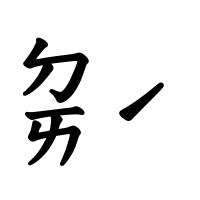
\includegraphics[height=1em]{圖/⿳⿳ㄉㄞˊ}}{tai5}
\rubybot{語 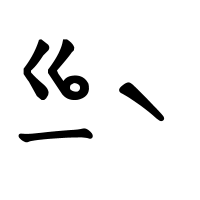
\includegraphics[height=1em]{圖/⿳⿳ㆣㄧˋ}}{gi2}

\emph{Traffic Light Systems} (\emph{TLSs}) are the major facilities for
managing transportations in urban areas nowadays. Traffic lights control the
priority of vehicles to pass intersections. Vehicles are thus forced to behave
in a stop-and-go manner according to traffic signals. Basically, the
\emph{Phase Timing Information} (\emph{PTI}) of each traffic light controls
its signal timing. PTI includes the traffic light cycle length and signal
transition time. It can be used in applications such as violation warning and
speed advisory for vehicles to pass an intersection. Further, by preventing
unnecessary braking and accelerating, fuel efficiency of vehicles can be
significantly improved. Indeed, the Travolution project \cite{Audio2011} ran
by Audi has shown that knowing PTI can help reduce 15\% of CO$_{\text{2}}$ emission.

However, due to many reasons, the PTI of traffic lights is unavailable to the
public. Not only PTI may change over time, but also TLSs may belong to
different authorities. In this paper, we adopt a \emph{crowdsoursing} approach
to discover the PTI of those target TLSs. Since traffic signals are the major
causes to influence traffic flows, it is possible to discover PTI from traffic
flow data. Smartphones embedded with GPS are used to detect the movement
features of vehicles. Thus any vehicle with a smartphone and our software can
serve as our probe car.
%and cloud service technologies
A remote cloud server is needed to run our PTI discovery algorithm. On the
smartphone side, a simple detection algorithm is needed to identify its
\emph{stop and go} (\emph{SG}) events in front of traffic lights. The cloud
server collects these events and uses a \emph{shockwave} technique
%cloud servers
to discover the PTI of those TLSs.
%in
%the form of cloud services.
Fig. \ref{fig:f_system_architecture} illustrates our
framework.\begin{figure}[pth]
\centerline{\includegraphics[angle=0, width=3.5in,keepaspectratio,clip]
{figures/f_system_architecture.eps}} \hfill\caption{Our crowdsourcing
framework for PTI discovery.}%
\label{fig:f_system_architecture}%
\end{figure}

PTI can enable many novel applications such as adaptive trip navigation, eco
driving advisory and red light advisory. When encountering an intersection,
drivers have to decide whether to pass or brake. From PTI, an advisory system
can provide advice for drivers to prevent unnecessary acceleration and braking
based on the red light residual time. In eco driving advisory, if long waiting
time is predicted, drivers may turn off idle engines. In fact, these can all
help driving safety at intersections. Recognizing the importance of PTI, US
and European transportation bureaus have advocated to integrate
\emph{Dedicated Short Range Communications} (\emph{DSRC}) with TLSs
\cite{Baldessari2007Communication}. However, this requires all traffic lights
and vehicles to install DSRC interfaces. In contrast, our crowdsoursing
approach requires nearly no infrastructure cost.

PTI can also be obtained in various other ways. The first thought is to use
the video cameras in vehicles to capture traffic signals. Such information, if
being captured, may be exchanged via \emph{Vehicular Ad hoc Networks}
(\emph{VANET}) \cite{Koukoumidis2011SignalGuru}. The video recognition
capability and the penetration issue are both crucial to this approach. The
second way is to rely on a centralized trusted office to collect all real-time
PTI from all TLS authorities \cite{RAMS2004}. For example, among 10,800
traffic lights in New York City, 4800 are still not connected to its central
system \cite{NewYork1998}.

In this work, we adopt the shockwave technique \cite{Lighthill1955KinematicI}%
\cite{Lighthill1955KinematicII} to find the PTI of TLSs. We regard the
%In this work, we propose a Smartphone-based Probe Car system (SPC)
%Cloud system (SPC-Cloud)
%to discover and share PTI.
%and vehicles
%are equipped with \emph{OnBoard Diagnostics} (\emph{OBD}) to provide useful
%driving information such as vehicle speed.
%Smartphones are equipped in vehicles to collect data from vehicles and sensing
%driving condition. In addition, smartphones report collected data to cloud
%servers via 3G/WiFi connections.
%Cloud
%Traffic information servers collect data from SPCs, mine traffic and road
%information, and then share the information via cloud services.
journey of a vehicle as a sequence of alternative stop and go events. A stop
event occurs when a vehicle reduces its speed to zero and a go event occurs
when it starts to move due to signal transition. We observe that the stop
events of vehicles in front of an intersection, when being put together, will
form a shockwave (called \emph{congestion wave}). Also, those go events can be
put together to form another shockwave (called \emph{relief wave}). From the
congestion and the relief waves of the same signal cycle, important PTI
parameters can be discovered. To conquer the problem when some essential
parameters are unknown, we also propose a way to collapse the SG events of
multiple signal cycles to reconstruct the congestion and relief waves. The
history of the shockwave theory in traffic management can be dated back to the
works in \cite{Lighthill1955KinematicI}\cite{Lighthill1955KinematicII}. In the
literature, shockwave models have been used in traffic flow reconstruction
\cite{Herrera2007Traffic}, queue length analyses \cite{Liu2009Real}%
\cite{Ban2011Real} and travel time estimation \cite{Skabardonis2008Real}.
However, these works rely on field sensors to collect traffic information,
making deployment and maintenance cost high. In this work, we propose to use
probe cars that may only represent a very low percentage of overall vehicles.
This makes reconstructing shockwaves more difficult. Also, since there may
exist lots of noise in the collected SG events, we propose
%and/or OBD
a Finite State Machine (FSM) to identify real SG events and remove potential noise.

Depending on the information that is given, we formulate the PTI discovery
problem in three versions. The first version assumes that the SG events are
caused by the same signal cycle of a traffic light. Therefore, the shockwave
technique can be directly applied to calculate the PTI information. The second
version relaxes the constraint such that the collected SG events are not
necessarily caused by the same signal cycle, but it still assumes that the
cycle length is known. We propose a \emph{folding} technique by collapsing
events over multiple cycles to virtually increase the number of SG events in a
cycle. The third version further removes the assumption of knowing the cycle
length. We believe that our solution is quite practical because probe cars
only need typical smartphones and only need to represent a very small
percentage of all vehicles on the roads. No extra roadside infrastructure and
no
%the traffic data are collected from SPCs as compared to the
%field located sensor-based method which is high cost in infrastructure
%deployment. In contrast to the probe car-based method, the SPCs provide well
%integration of smartphones and vehicles for mobile sensing and wireless
%communications.
complicated algorithms (such as video recognition) are required. Our folding
technique tolerates location errors and small samples due to shortage of probe
cars. This is possible because the PTI of a TLS is not expected to change
rapidly over a short period of time. Our experiments show that using GPS is
sufficient to detect most of the SG events. This implies that if OBDs and IMUs
are adopted, the detection accuracy can be further improved.
%Due to the delay and drifting nature and low
%sampling rate (usually 1 Hz) of GPS, OBD-based solution outperforms GPS-based
%one.
In our experiments, when the penetration rate is $1.2\%$ and 9 SG event pairs
are collected, the \emph{Root Mean Square Error} (\emph{RMSE}) of the measured
cycle length, red light transition time, red light phase length, green light
transition time, and green light phase length are $2.3$ seconds, $7.8$
seconds, $5.7$ seconds, $8.2$ seconds and $5.2$ seconds, respectively. This
verifies the potential of our framework.
%4) the
%proposed framework has the potential for mass deployment with the help of
%cloud computing technologies.
%The traffic data collection method can be categorized to field-located based
%methods \cite{Liu2009Real}\cite{Skabardonis2008Real}%
%\cite{Wu2010Identification}\cite{Wu2010Empirical} and probe-car based methods
%\cite{Herrera2007Traffic}\cite{Ban2011Real}\cite{Herrera2010Evaluation}
%methods. The field located sensor-based method collects traffic data from
%field located sensors such as loop detectors and vehicle detectors.
%Skabardonis and Geroliminis \cite{Skabardonis2008Real} developed an analytical
%model for travel time estimation in signalized arterials based on data
%collected from the loop detectors. Liu \textit{et al.} \cite{Liu2009Real}
%discovered a \emph{Queue-Over-Detector} (QOD) problem in the traditional
%input-output approach for queue length estimation in signalized road segments,
%and used high resolution traffic signal data with data collected by loop
%detectors to estimate time-dependent queue length. Followed by Wu \textit{et
%al.} \cite{Wu2010Identification}, \emph{Oversaturated Severity Index} (OSI) is
%defined for quantifying the effects of spillovers, and further separated to
%temporal OSI and spatial OSI according to how the OSI affects in temporal and
%spatial dimensions. After that, the QOD problem in signalized arterials was
%further discussed in \cite{Wu2010Empirical}, they showed that the QOD can
%significantly affect the accuracy of \emph{Arterial Fundamental Diagram} (AFD)
%and concluded that after removing the QOD effects, one can use AFD to
%interpret the traffic flow in signalized arterials. The high cost in
%infrastructure deployment is the main issue in the field located sensor-based method.
%On the other hand, the probe car-based method tried to utilize new mobile
%sensing technologies, such as GPS tracking logs, for other means of traffic
%data collection. In \cite{Herrera2007Traffic}, Herrera \textit{et al.}
%proposed to incorporate GPS tracking logs with data collected from loop
%detectors for traffic flow reconstruction. However, they did not discuss the
%penetration rate of GPS in vehicles, which directly affects the accuracy of
%the estimated traffic flow. In \cite{Ban2011Real}, Ban \textit{et al.} used
%travel time between intersections from GPS tracking logs, and developed an
%analytical model from the concept of \emph{Queue Rear No-delay Arrival Time}
%(QRNAT). In \cite{Herrera2010Evaluation}, they performed a field trial to show
%that a $2-3\%$ penetration of GPS in vehicles is enough to provide accurate
%measurement data for traffic flow estimation. The high cost and tedious
%installation for embedded sensors make the probe car-based method not popular
%in practical applications.
%\section{System Architecture}
%\label{sec:System_Architecture}
%The proposed system is composed of two components including Smartphone Probe
%Cars (SPCs) and Traffic Information (TI) servers. Fig.
%\ref{fig:f_system_architecture} illustrates the architecture of the proposed
%system. \begin{figure}[pth]
%\centerline{\includegraphics[angle=0, width=3.2in,keepaspectratio,clip]
%{figures/f_system_architecture.eps}} \hfill\caption{System architecture.}%
%\label{fig:f_system_architecture}%
%\end{figure}
%The SPCs consist of vehicles equipped with smartphones for traffic event
%detection.
%%OBD is optional to provide real-time vehicle
%%states for improving the accuracy of SG event detection.
%The detected traffic events can be reported to the TI servers by online or
%batch modes depending on the wireless connections. The SPCs can display
%traditional navigation information such as UI, digital maps, position
%information of the SPC and the nearby traffic light in the digital maps. In
%addition, advanced traffic light advisory information such as red light
%residual time and green light residual time, can be also displayed by the
%SPCs. Drivers can make proper decisions to avoiding unnecessary acceleration
%and braking based on the advanced traffic light advisory information.
%The TI servers contain a Geographic Information System DataBase (GIS DB) for
%digital map information, an SG event DataBase (SG DB) for SG event collection
%and a PTI DataBase (PTI DB) for the\ PTI. The PTI can be shared to SPCs or
%queried by PCs via Internet for the advanced traffic light advisory information.
%\subsection{SPC Subsystem}
%An SPC is a dynamic integration of a smartphone and a vehicle. Embedded
%sensors of smartphones or onboard sensors of vehicles are used to detect
%traffic events such as stop events and go events. The detected events are
%reported to the TI servers via wireless connections.
%%If an OBD is
%%available in a vehicle, it can be adopted as an assistance device to improve
%%the accuracy of SG event detection.
%The SPC collects raw data such as position and corresponding timestamp
%information and displays traffic information provided from the TI servers. As
%illustrated in the right side of Fig. \ref{fig:f_system_modules}, there are
%three modules in the SPC subsystem including an SG event detection module, an
%event report module and an advisory module. \begin{figure}[pth]
%\centerline{\includegraphics[angle=0, width=3.2in,keepaspectratio,clip]
%{figures/f_system_modules.eps}} \hfill\caption{System modules.}%
%\label{fig:f_system_modules}%
%\end{figure}The SG event detection module detects SG events based on the
%driving speed reported from GPS.
%%and/or OBD in case OBD is available.
%The event report module uploads the detected SG events to the\ TI servers by
%online mode if network connections are available or batch mode, otherwise. The
%advisory module displays traditional navigation information such as UI,
%digital maps, position information of the SPC and the nearby traffic light in
%the digital maps. In addition, advanced traffic light advisory information
%obtained via cloud services such as red light residual time, green light
%residual time
%%, predicted waiting time
%and minimum recommended speed to cross the intersection, is also displayed by
%the advisory module.
%%The predicted
%%waiting time is calculated based on the stopped position and the PTI.
%The minimum recommended speed to cross the intersection is calculated by
%dividing the distance of the stopped position to the position of traffic light
%at the intersection by the green light residual time. Drivers can make proper
%decisions to avoiding unnecessary acceleration and braking based on the
%advanced traffic light advisory information.
%\subsection{TLI Cloud Subsystem}
%The TI servers collects events from the SPCs, stores events in databases,
%mines traffic information from the events and provides cloud services for
%sharing traffic light information. The TI servers have four modules including
%an event collection module, a storage module, a PTI mining module and a
%sharing module as depicted in the left side of Fig. \ref{fig:f_system_modules}%
%. The event collection module collects SG events reported by the SPCs. The
%storage module stores traffic events and PTI in databases, and provides
%traffic events for PTI mining, Geographic Information (GI) and PTI for sharing
%information. The PTI mining module mines the PTI and shockwave equations from
%the SG events. The sharing module shares PTI and geographic information to the
%advisory module in the SPCs.
%In addition, due to
%the delay nature and low sampling rate of GPS, the speed reported by GPS is
%usually with a varied time offset. The delay issue can be alleviated by
%assistance of OBD which provides real-time vehicle states including driving speed.


The rest of this paper is organized as follows. Chapter
\ref{cha:related-works} covers some preliminaries.
%In Section
%\ref{sec:System_Architecture}, the proposed system architecture is presented.
The three versions of the PTI discovery problem are formulated in Chapter
\ref{cha:problem_formulation}. Chapter \ref{cha:solutions} presents our
solutions based on the shockwave approach. Our field trial and simulation
results are provided in Chapter \ref{cha:simulation-results} and
\ref{cha:Impement}. Conclusions and future works are drawn in Chapter
\ref{cha:Conclusions}.

\chapter{Related Works}

\label{cha:related-works}

Below, we first review some backgrounds about Probe Car Sensing and TLSs,
followed by some preliminaries of the shockwave theory.

\section{Traffic Light Systems}

The schedule of a TLS constitutes a sequence of signal cycles and each
consisting multiple phases \cite{Banks2002Transportation}. In general, such
schedule can be categorized as \emph{fixed-time} and \emph{dynamic-time} modes
\cite{Banks2002Transportation}. Under the fixed-time mode, the settings of
phase lengths and cycle lengths are fixed according to different durations of
a day (such as off-peak, am-peak, pm-peak, holiday-peak, etc.) For example,
about 96\% of the TLSs in the US are operated under the fixed-time mode
\cite{Koukoumidis2011SignalGuru}. The dynamic-time mode is proposed to
optimally adjust phase and cycle lengths according to real-time traffic
conditions. To operate, such TLSs rely on detection loops installed on the
roads. The Sydney Coordinated Adaptive Traffic System (SCATS) is an example of
such TLSs \cite{Akcelik2001SCARTS}.

There are many works and projects related to the PTI discovery problem. The
Travolution project by Audi proposes to adopt wireless communications in TLSs
and vehicles. Vehicles can directly obtain PTI from nearby traffic lights. It
is reported that by providing PTI to drivers, both air pollution and fuel
efficiency are improved significantly by 15\% and 17\% \cite{Audio2011}.
However, the deployment cost is non-trivial. In\textit{ }%
\cite{Koukoumidis2011SignalGuru}, a system consisting of cars is\ proposed to
estimate the PTI of the fixed-time and dynamic-time modes TLSs. The
transitions of traffic signals are extracted from the videos recorded by the
cameras of smartphones. The PTI under the fixed-time mode is estimated by
looking up a preinstalled database from the traffic management center, whereas
the PTI under the dynamic-time mode is estimated by a support vector machine
trained from historical data obtained from the traffic management center. This
approach is constrained by the video recognition capability (such as the
light-of-sight issue), the penetration of vehicles participating in the
application and the assumption of preinstalled historical database.

\begin{figure}[pth]
\centerline{\includegraphics[angle=0, width=3.2in,keepaspectratio,clip]
{figures/f_fd.eps}} \hfill\caption{Propagation of two shockwaves in a
signalized road segment.}%
\end{figure}

\section{Shockwaves Research}

Shockwaves theory has been first proposed in 1955 in
\cite{Lighthill1955KinematicI}\cite{Lighthill1955KinematicII}.After that,
\cite{Richard1956Shock} also investigate shockwaves that appeared in highway.
Shockwaves is the phenomenon between two different traffic flows. In their
research, the density, flow and speed of traffic change respect to time and
space domain. A shockwave appears when two flows with different speeds and
densities meet each other.When two different flows attach together, the
vehicle's which at the edge between two different flows will rapidly change.
And this phenomenon will spread as a wave form to other vehicles. In hence,
they use \textquotedblleft shockwaves\textquotedblright\ as this phenomenon
and \cite{Stephanopoulos1979Modeling}\cite{Michalopoulos1981application} model
this phenomenon in traffic. In urban, there are two shockwaves appearing in a
signalized road segment.In \cite{Chuang2013Crowdsourced}, a preliminary result
of the shockwave model in signalized intersections on traffic information
mining was studied. The propagation of shockwaves in a signalized road segment
can be depicted by a time-position diagram as shown in Fig.
\ref{fig:f_application_shock}. Each dash arrow represents vehicles'
tims-position relation with respect to the road segment. The trajectories of
vehicles consist of three different speed. On encountering a red sign,
vehicles gradually stop, forming a \emph{congestion wave}. On the sign turning
to green, these vehicles start to move, forming a \emph{relief wave}. Note
that both waves are caused by the changes of speeds of flows. A fundamental
observation of our work is that as long as the arrival pattern and signal
pattern remain unchanged, the shockwave patterns can be identified and hence
the PTI of the TLS.\ss 

\chapter{Problem Formulation}

\label{cha:problem_formulation}

In this chapter, we formulate the PTI discovery problem in three versions. The
trip of a vehicle is regarded as a sequence of alternative \emph{halt} and
\emph{move} periods separated by \emph{stop} and \emph{go} events at same
locations. A stop event indicates the transition from a move period to a halt
period, and a go event indicates that from a halt period to a move period. A
stop event happening at time $t^{s}$ in position $p^{s}$ of a vehicle is
denoted by $\left(  t^{s},p^{s}\right)  $, and a go event happening at time
$t^{g}$ in position $p^{g}$ is denoted by $\left(  t^{g},p^{g}\right)  $. We
say that a stop event and a go event are an \emph{SG event pair} if they are
the beginning and the ending events, respectively, of the same halt period of
a vehicle's trip. Note that if a GPS is used, it may happen that $p^{s}$ may
be slightly different from $p^{g}$ due to the location drifting problem. We
will take the average of the GPS measurements over the period $\left[
t^{s},t^{g}\right]  $ as the position. Also note that we only need a
participating vehicle to report its SG event pairs without releasing its ID.
So there is no privacy concern.

The schedule of a TLS is regarded as two sequences $\left\{  R_{i}\right\}  $
and $\left\{  G_{i}\right\}  $ such that $R_{i}$ and $G_{i}$ are the time of
its $i$th transitions to red and green, respectively. Without loss of
generality, we assume that $G_{i}$ follows $R_{i}$ immediately, \textit{i.e.},
$R_{i}<G_{i}<R_{i+1}<G_{i+1}$, for all $i$. The interval $\left[
R_{i},R_{i+1}\right]  $ is called a \emph{signal cycle}.\ We consider the
fixed-time mode such that $R_{i+1}=R_{i}+T$ and $G_{i+1}=G_{i}+T$ for all $i$,
where $T$ is a constant cycle length. We assume that the arrival and departure
rates of vehicles remain constant over a short period of time (for example, if
it is stable within $5$ to $10$ signal cycles, our approach should work).
Based on these assumptions, we define three versions of the PTI discovery problem.

\begin{problem}
\label{prob:ver1}From probe cars, we have collected a sequence $S=\left\{
s_{1},s_{2},\cdots,s_{n}\right\}  $ of stop events and a sequence $G=\left\{
g_{1},g_{2},\cdots,g_{n}\right\}  $ of go events associated with a traffic
light such that $s_{j}$ and $g_{j}$ are a SG event pair, $j=1,...,n$. Assuming
that these event pairs are all caused by the same signal cycle $\left[
R_{i},R_{i+1}\right]  $ and the cycle length $T$ is known, the problem is to
find the transition time $R_{i}$ and $G_{i}$.
\end{problem}

\begin{problem}
\label{prob:ver2}From probe cars, we have collected a sequence $S=\left\{
s_{1},s_{2},\cdots,s_{n}\right\}  $ of stop events and a sequence $G=\left\{
g_{1},g_{2},\cdots,g_{n}\right\}  $ of go events associated with a traffic
light such that $s_{j}$ and $g_{j}$ are a SG event pair, $j=1,...,n$. Assuming
that these event pairs are caused by multiple signal cycles and the cycle
length $T$ is known, the problem is to find the sequences $\left\{
R_{i}\right\}  $ and $\left\{  G_{i}\right\}  $.
\end{problem}

\begin{problem}
\label{prob:ver3}From probe cars, we have collected a sequence $S=\left\{
s_{1},s_{2},\cdots,s_{n}\right\}  $ of stop events and a sequence $G=\left\{
g_{1},g_{2},\cdots,g_{n}\right\}  $ of go events associated with a traffic
light such that $s_{j}$ and $g_{j}$ are a SG event pair, $j=1,...,n$. The
problem is to find the cycle length $T$ and the sequences $\left\{
R_{i}\right\}  $ and $\left\{  G_{i}\right\}  $.
\end{problem}

Clearly, more information is provided to Problem \ref{prob:ver1} as compared
to Problem \ref{prob:ver2}, and so is Problem \ref{prob:ver2} as compared to
Problem \ref{prob:ver3}. Below, we make some observations to help explain the
nature of these problems. Fig. \ref{fig:SG_shockwaves}(a) illustrates some
collected SG events drawn in a time-position graph. For Problem
\ref{prob:ver1}, only the events within a single cycle are given. If these
collected events are dense enough, a linear trend may exist in the graph for
both the congestion and the relief waves. These waves can thus be expressed by
equations
\begin{align*}
L^{s}  &  :p_{i}^{s}\doteqdot\alpha^{s}t_{i}^{s}+\beta^{s}\\
L^{g}  &  :p_{i}^{g}\doteqdot\alpha^{g}t_{i}^{g}+\beta^{g}%
\end{align*}
$\frac{{}}{{}}$where $\alpha^{s}$ and $\alpha^{g}$ are constants proportional
to the arrival and departure rates of vehicles, respectively, and $\beta^{s}$
and $\beta^{g}$ are constants. To find $L^{s}$ and $L^{g}$, a Least Square
Method (LSM) may be applied. If we regard the position of the traffic light as
the origin, then $-\beta^{s}/\alpha^{s}$ is the red light transition time and
$-\beta^{g}/\alpha^{g}$ is the green light transition time. So, $\left(
-\beta^{g}/\alpha^{g}\right)  -\left(  -\beta^{s}/\alpha^{s}\right)  $ is the
red light phase length and $T-\left(  -\beta^{g}/\alpha^{g}\right)  $ is the
green light phase length.\begin{figure}[pth]
\centerline{\includegraphics[angle=0, width=6in,keepaspectratio,clip]
{figures/f_stop_go_shockwaves.eps}} \hfill\caption{An example of collected SG
events in a signalized road segment.}%
\label{fig:SG_shockwaves}%
\end{figure}

For Problem \ref{prob:ver2}, since traffic flows are stable, the wave
equations should have similar slopes. Also, since $T$ is known, we can
collapse events over the temporal dimension by either adding or subtracting
the multiple of $T$ to the time component of events such that all events are
inside a single cycle. This virtually increases the number of events for
finding equations $L^{s}$ and $L^{g}$. Fig. \ref{fig:SG_shockwaves}(b) shows
the folding result of Fig. \ref{fig:SG_shockwaves}(a). This is why our
approach only requires a very small portion of probe cars over all vehicles.

For Problem \ref{prob:ver3}, since $T$ is unknown, we need to find its value.
Since the wave equations repeats every cycle, one possibility is to use
typical techniques in digital signal processing such as the Fourier
transformation to find $T$. However, when the number of samples per cycle is
too low, such techniques may still fail (for example, some cycles may have no
samples). Fortunately, the time difference between two apart stop/go events is
likely to fall within a multiple of $T$ with small variation. This sheds some
light to find $T$ by a real-value Greatest Common Divisor (GCD) from the
multiples. We will propose a clustering technique to find $T$ and remove
potential noises in this approach.

\chapter{臺語介紹}

\label{cha:solutions}

In this chapter, we present our solutions to the PTI discovery problem, which
consist of four modules: SG event detection, shockwave identification, event
folding and cycle length discovery. How to combine these modules to solve our
problems is shown in Fig. \ref{fig:f_solution_framework}. The SG event
detection module is required for all problems. Problem \ref{prob:ver1} only
requires the shockwave identification module. For Problem \ref{prob:ver2}, the
event folding module is further needed to virtually increase the number of
events (\textit{i.e.}, data density) per signal cycle. For Problem
\ref{prob:ver3}, the cycle length discovery module is further applied to mine
the cycle length. Note that for Problem \ref{prob:ver2} and \ref{prob:ver3},
the event folding module and the shockwave identification module will be
repeated for each reference point (refer to Chapter
\ref{sec:folding_technique}).\begin{figure}[pth]
\centerline{\includegraphics[angle=0, width=3.2in,keepaspectratio,clip]
{figures/f_solution_framework.eps}} \hfill\caption{Solutions to the three
versions of the PTI discovery problem.}%
\label{fig:f_solution_framework}%
\end{figure}

\section{Stop-Go Event Detection Module}

\bigskip

\label{sec:detect_SG_events}

\begin{figure}[pth]
\centerline{\includegraphics[angle=0, width=3.5in,keepaspectratio,clip]
{figures/f_GPS_FSM.eps}} \hfill\caption{The finite state machine for SG event
detection.}%
\label{fig:f_GPS_FSM}%
\end{figure}

The input to this module is trips of probe cars. Each trip consists of a
sequence of velocity-position pairs collected by a probe car. Note that the
knowledge of a vehicle's position traces does not necessarily imply the
knowledge of its velocity traces due to GPS locations errors, and vice versa.
Since a vehicle may move slowly in a stop-and-go manner before it actually
stops in front of a red sign, we propose a \emph{Finite State Machine} (FSM)
as shown in Fig. \ref{fig:f_GPS_FSM} to model the state transition of a
vehicle. In our FSM, there are three states: MOVE, HALT, and STOPPING. The
first two states are self-explained. The STOPPING state is to model the grey
area during the stop-and-go periods. We control the transition among these
states by two parameters, $V_{th}$ and $T_{th}$. The former is a velocity
threshold, while the later is a time duration threshold. Let $v$ denote the
current speed of the vehicle and $tick$ denote the duration after it enters
the STOPPING state. The vehicle is in the MOVE state whenever $v\geq V_{th}$.
In the MOVE state, it goes to the STOPPING state when $v<V_{th}$ and starts
counting the duration by $tick$. Whenever $v\geq V_{th}$, it returns to MOVE
and resets $tick$. In the STOPPING state, when $tick>T_{th}$, it transits to
the HALT state. In the HALT state, once $v\geq V_{th}$, it goes to the MOVE
state and immediately reports a stop event and a go event with $t^{s}$ and
$t^{g}$ set to the time when it transits into and out of the HALT state,
respectively, and $p^{s}$ and $p^{g}$ both set to the centroid of the measured
locations.
%The details of
%the GPS-based SG event detection algorithm are depicted in PROCEDURE
%\ref{alg:event_detect}. \floatname{algorithm}{PROCEDURE}
%\renewcommand{\algorithmicrequire}{\textbf{INPUT}}
%\renewcommand{\algorithmicensure}{\textbf{BEGIN}} \begin{algorithm}
%\caption{EventSearch}
%\begin{algorithmic}[1]
%\ENSURE
%\STATE $state=$STOP; $tick=0$; $i=0$;
%\WHILE{there is a datum in GPS buffer}
%\STATE get the $i$-th GPS datum from GPS buffer;
%\STATE $v_{i}$: the speed of the $i$th GPS datum;
%\IF{$v_{i}\geq toStop$}
%\IF{$state=$STOP}
%\STATE Report a go event;
%\ENDIF
%\STATE $state=$GO;
%\ELSE
%\IF{$state=$GO}
%\STATE $tick=0$;
%\STATE $state=$STOPPING;
%\STATE Keep the location and time;
%\ELSIF{$state=$STOPPING}
%\STATE $tick=tick+1$;
%\IF{$tick=QuarDur$}
%\STATE Report a stop event;
%\STATE $state=$STOP;
%\ENDIF
%\ENDIF
%\ENDIF
%\STATE $i=i+1$;
%\ENDWHILE
%\end{algorithmic}\label{alg:event_detect}
%\end{algorithm}
Note that a vehicle following the FSM does not necessarily completely stop and
may move in a slow speed in the HALT state.

%The inaccuracy, drifting and non-instant nature and low sampling rate (about
%1Hz) of GPS all make the GPS-based detection algorithm not precise. To address
%this phenomenon, the driving speed obtained from OBD is compared with the
%speed from GPS.
%%OBD is used to obtain driving speed instead of GPS.
%%The flow chart of
%%the proposed OBD-refinement algorithm is depicted in Fig.
%%\ref{fig:f_obd_tuning_flow}. Let $v_{i}$ be the driving speed at time $t_{i}$.
%%Now, if a stop event $\left(  t^{s},p^{s}\right)  $ is detected by the event
%%detection algorithm, the OBD-refinement algorithm is triggered to scan the
%%driving speed $v_{i}$ backward from time $t^{s}$ to time $t^{s}-QuarDur$ to
%%find a speed which is greater then $toStop$. Then, the time and position
%%related to the first found speed are reported to replace the original stop
%%event as shown in line 2 to 8 in PROCEDURE \ref{alg:OBD-refine}. Similarly, if
%%a go event $\left(  t^{g},p^{g}\right)  $ is reported by the GPS-based
%%detection algorithm, the OBD-refinement algorithm is triggered to scan the
%%driving speed forward from time $t^{g}-2QuarDur$ to time $t^{g}$ to find a
%%speed which is less then $toStop$. Then, the time and position related to the
%%first found speed are reported to replace the original go event as shown in
%%line 9 to 14 in PROCEDURE \ref{alg:OBD-refine}. However, no matter for the
%%stop or go event, if there are no such speeds found, the event is not updated.
%%The details of the proposed OBD-refinement algorithm is given in PROCEDURE
%%\ref{alg:OBD-refine}. \floatname{algorithm}{PROCEDURE}
%%\renewcommand{\algorithmicrequire}{\textbf{INPUT}}
%%\renewcommand{\algorithmicensure}{\textbf{BEGIN}} \begin{algorithm}
%%\caption{OBD-refinement}
%%\begin{algorithmic}[1]
%%\ENSURE
%%\STATE $state$: the vehicle state
%%\IF{$state=$GO}
%%\FOR{$i=t^{s}-2QuarDur$ to $t^{s}$}
%%\IF{$v_{i} > toStop$}
%%\RETURN the position and time related to $v_{i}$
%%\ENDIF
%%\ENDFOR
%%\ELSE
%%\FOR{$i=t^{s}$ to $t^{s}-QuarDur$}
%%\IF{$v_{i} < toStop$}
%%\RETURN the position and time related to $v_{i}$
%%\ENDIF
%%\ENDFOR
%%\ENDIF
%%\RETURN No update
%%\end{algorithmic}\label{alg:OBD-refine}
%%\end{algorithm}\begin{figure}[pth]
%%\centerline{\includegraphics[angle=0, width=3.5in,keepaspectratio,clip]
%%{figures/f_obd_tuning_flow.eps}} \hfill\caption{The flow chart of the
%%OBD-refinement algorithm.}%
%%\label{fig:f_obd_tuning_flow}%
%%\end{figure}
%Fig. \ref{fig:f_wave_gps_speed} depicts an instance of the time domain
%waveforms of GPS and OBD tracking logs and the SG events reported by the
%proposed algorithms. \begin{figure}[pth]
%\centerline{\includegraphics[angle=0, width=3.5in,keepaspectratio,clip]
%{figures/f_wave_gps_speed.eps}} \hfill\caption{A waveforms from GPS tracking
%logs with a SG event pair.}%
%\label{fig:f_wave_gps_speed}%
%\end{figure}In the figure, the (blue) line marked with diamonds and the (red)
%line marked with squares are the speed reported by OBD and GPS, the x-axis is
%time line in $second$ and the y-axis is the scale of speed in $Km/hr$. The
%zone between two vertical solid lines is the stopped duration detected by OBD
%and the zone between two vertical dash line is the stopped duration detected
%by GPS. The thresholds used in the detection algorithms, including $toStop$
%and $QuarDur$ are set to $2.7$ $Km/hr$ and $2$ seconds, respectively. The stop
%and go events are respectively marked at $30221.1$ second and $30230.1$ second
%by the GPS-based detection algorithm and at $30222.1$ second and $30229.1$
%second by the OBD-based detection algorithm. We can see that GPS has a delayed
%response and therefore the SG events reported by the GPS-based detection
%algorithm is usually behind the events detected by OBD.
%%However, from the example provided in Fig.
%%\ref{fig:f_wave_gps_speed}, we can see that the delay problem of GPS can be
%%significantly corrected by utilizing OBD to fine tune the reported stop and go events.


\section{Shockwave Identification Module}

\bigskip

\label{sec:stop_go_shockwaves}

Recall the observations in Chapter \ref{cha:problem_formulation}. We need to
find the constants $\alpha^{s}$, $\beta^{s}$, $\alpha^{g}$ and $\beta^{g}$ to
approximate the stop events $\left\{  s_{1},s_{2},\cdots,s_{n}\right\}  $ and
the go events $\left\{  g_{1},g_{2},\cdots,g_{n}\right\}  $ such that%
\begin{align*}
p_{i}^{s}  &  \doteqdot\alpha^{s}t_{i}^{s}+\beta^{s}\\
p_{i}^{g}  &  \doteqdot\alpha^{g}t_{i}^{g}+\beta^{g}%
\end{align*}
for all $i=1,...,n$. We apply the Least Square Method (LSM) by setting the
matrices:
\begin{align*}
\mathbb{T}^{s}  &  =\left[
\begin{array}
[c]{cc}%
t_{1}^{s} & 1\\
t_{2}^{s} & 1\\
\vdots & \vdots\\
t_{n}^{s} & 1
\end{array}
\right]  \text{, }\mathbf{p}^{s}=\left[
\begin{array}
[c]{c}%
p_{1}^{s}\\
p_{2}^{s}\\
\vdots\\
p_{n}^{s}%
\end{array}
\right]  \text{, }\mathbf{x}^{s}=\left[
\begin{array}
[c]{c}%
\alpha^{s}\\
\beta^{s}%
\end{array}
\right]  \text{,}\\
\mathbb{T}^{g}  &  =\left[
\begin{array}
[c]{cc}%
t_{1}^{g} & 1\\
t_{2}^{g} & 1\\
\vdots & \vdots\\
t_{n}^{g} & 1
\end{array}
\right]  \text{, }\mathbf{p}^{g}=\left[
\begin{array}
[c]{c}%
p_{1}^{g}\\
p_{2}^{g}\\
\vdots\\
p_{n}^{g}%
\end{array}
\right]  \text{, and }\mathbf{x}^{g}=\left[
\begin{array}
[c]{c}%
\alpha^{g}\\
\beta^{g}%
\end{array}
\right]  \text{.}%
\end{align*}
We have two linear systems: $\mathbb{T}^{s}\mathbf{x}^{s}=\mathbf{p}^{s}$ and
$\mathbb{T}^{g}\mathbf{x}^{g}=\mathbf{p}^{g}$. It follows that
\begin{align*}
\left(  \mathbb{T}^{s}\right)  ^{T}\mathbb{T}^{s}\mathbf{x}^{s}  &  =\left(
\mathbb{T}^{s}\right)  ^{T}\mathbf{p}^{s}\text{ and}\\
\left(  \mathbb{T}^{g}\right)  ^{T}\mathbb{T}^{g}\mathbf{x}^{g}  &  =\left(
\mathbb{T}^{g}\right)  ^{T}\mathbf{p}^{g}\text{.}%
\end{align*}
Hence,
\begin{align}
\mathbf{x}^{s}  &  =\left(  \left(  \mathbb{T}^{s}\right)  ^{T}\mathbb{T}%
^{s}\right)  ^{-1}\left(  \left(  \mathbb{T}^{s}\right)  ^{T}\mathbf{p}%
^{s}\right)  \text{ and}\label{eq:e_equation_congestion}\\
\mathbf{x}^{g}  &  =\left(  \left(  \mathbb{T}^{g}\right)  ^{T}\mathbb{T}%
^{g}\right)  ^{-1}\left(  \left(  \mathbb{T}^{g}\right)  ^{T}\mathbf{p}%
^{g}\right)  \text{.} \label{eq:e_equation_relief}%
\end{align}
%Furthermore, Let $\overline{p}_{i}$ be the position where the vehicle stops.
%Ideally, we may assume $\overline{p}_{i}=p_{i}^{s}=p_{i}^{g}$. However, due to
%the drift problem and the inaccurate of the detection algorithm, it is the
%common case in which $p_{i}^{s}\neq p_{i}^{g}$. We denote $\overline{p}_{i}$
%the average of $p_{i}^{s}$ and $p_{i}^{g}$. In addition, let $\Delta
%t_{i}=t_{i}^{g}-t_{i}^{s}$ be the waiting time of the vehicles. A waiting time
%equation $L^{\Delta}:\overline{p}_{i}=\alpha^{\Delta}\Delta t_{i}%
%+\beta^{\Delta}$ can be obtained by applying the same method to $\Delta t_{i}$
%and $\overline{p}_{i}$. If a stop position $\overline{p}$ is given, the
%waiting time can be estimated by $\frac{\overline{p}-\beta^{\Delta}}%
%{\alpha^{\Delta}}$.


\section{Event Folding Module}

\label{sec:folding_technique}

For Problems \ref{prob:ver2} and \ref{prob:ver3}, the stop events and go
events may be caused by multiple signal cycles. Therefore, it is impossible to
approximate these shockwaves by one single linear function. Also, we have
mentioned the problems of sparse stop/go events (due to low traffic loads or
low penetration rate of probe cars) and GPS location errors. This module takes
any SG event pair as a \emph{reference point} and tries to "fold" all SG
events pairs into one signal cycle with respect to the reference point. It
helps improve data density and thus can potentially filter out noise. It
relieves the above problems while construct a "legal" set of SG event pairs
that can be used as inputs to the shockwave identification module. In this
module, \ we have to choose a SG event pair as the reference point. This
module is run iteratively for each SG event pair (this is reflected by the
loops in Fig. \ref{fig:f_solution_framework}). Then the most suitable folded
event sets are selected. Below, we present the event folding module by
assuming event pair $\left(  s_{r},g_{r}\right)  ,$ $1\leq r\leq n$, as the
given reference point. The basic idea is that in each signal cycle, the same
congestion and relief waves will re-appear with a period of $T$ when the
arrival rate of vehicles is stable. Based on this observation, we will convert
sequences $S=\left\{  s_{1},s_{2},\cdots,s_{n}\right\}  $ and $G=\left\{
g_{1},g_{2},\cdots,g_{n}\right\}  $ into $S^{\prime}=\left\{  s_{1}^{\prime
},s_{2}^{\prime},\cdots,s_{n}^{\prime}\right\}  $ and $G^{\prime}=\left\{
g_{1}^{\prime},g_{2}^{\prime},\cdots,g_{n}^{\prime}\right\}  $, respectively,
such that $S^{\prime}$ and $G^{\prime}$ will fall within a signal cycle. Here
$s_{r}$ and $g_{r}$ are converted to $s_{r}^{\prime}$ and $g_{r}^{\prime}$,
respectively, without change. For each $s_{i}=\left(  t_{i}^{s},p_{i}%
^{s}\right)  ,$ $i\neq r$, it is converted to $s_{i}^{\prime}=\left(
t_{i}^{s\prime},p_{i}^{s\prime}\right)  $ as follows.

\begin{enumerate}
\item Set $p_{i}^{s\prime}:=p_{i}^{s}$.

\item Subtract or add a multiple of $T$ to $t_{i}^{s}$ by finding an integer
$m$ such that $t_{i}^{s}+mT$ falls in the range $\left(  t_{r}^{s}-T,t_{r}%
^{s}+T\right)  $. Note that $\left(  t_{r}^{s}-T,t_{r}^{s}+T\right)  $ covers
a time span of $2T$. Ideally, there may exist only one $m$ such that
$t_{i}^{s}+mT\in\left(  t_{r}^{s}-T,t_{r}^{s}+T\right)  $ and we will set
$t_{i}^{s\prime}:=t_{i}^{s}+mT$. However, in most cases, there are two $m$s
meeting this condition. We pick one as follows.

\begin{itemize}
\item If $d\left(  p_{r}^{s},p_{i}^{s\prime}\right)  \leq\eta$, then the $m$
such that $\left\vert t_{r}^{s}-\left(  t_{i}^{s}+mT\right)  \right\vert $ is
smaller is selected, where $d\left(  {}\right)  $ gives the distance between
two positions and $\eta$ is a location error threshold.

\item Otherwise, we connect point $\left(  t_{r}^{s},p_{r}^{s}\right)  $ with
the two potential points given by $\left(  t_{i}^{s}+mT,p_{i}^{s\prime
}\right)  $ to form two lines. The one which has a negative slope is selected.
\end{itemize}

\item Set $t_{i}^{s\prime}=t_{i}^{s}+mT$ with the selected $m$.
\end{enumerate}

Similarly, for each $g_{i}=\left(  t_{i}^{g},p_{i}^{g}\right)  ,$ $i\neq r$,
it is converted to $g_{i}^{\prime}=\left(  t_{i}^{g\prime},p_{i}^{g\prime
}\right)  $ by the same steps. To understand the above conversion, we take
Fig. \ref{fig:f_folding} as an example. Stop event $s_{r}$ is the reference
point and stop events $s_{1},s_{2}$ and $s_{3}$ are events in other cycles.
Fig.\ref{fig:f_folding} (a) shows the ideal situation, where each of $s_{1}$,
$s_{2}$ and $s_{3}$ can find a unique $m$ for its conversion. It can be seen,
$s_{r},s_{1}^{\prime},s_{2}^{\prime}$ and $s_{3}^{\prime}$ form a perfect line
(\textit{i.e.}, shockwave). On the other hand, Fig.\ref{fig:f_folding} (b)
shows the situation where there are location errors. For $s_{1}$, there are
two candidates, $s_{1}^{\prime}$ and $s_{1}^{\prime\prime}$. Since the line
crossing $s_{r}$ and $s_{1}^{\prime}$ has a negative slope, $s_{1}^{\prime}$
is selected. For $s_{2}$, $s_{2}^{\prime}$ is selected for the same reason.
For $s_{3}$, since the locations where $s_{r}$ and $s_{3}$ are within a
distance of $\eta$, the one which is temporally closer to $s_{r}$
(\textit{i.e.}, $s_{3}^{\prime}$) is selected. It can be seen that such a
conversion pulls the folded events closer to the shockwave passing $s_{r}$.
Intuitively, when an event appears spatially close to the reference point, the
conversion will be based on the temporal proximity; otherwise, the conversion
will be based on both temporal and spatial information (\textit{i.e.}, slope).

\begin{figure}[pth]
\centerline{\includegraphics[angle=0, width=6.5in,keepaspectratio,clip]
{figures/f_folding.eps}} \hfill\caption{An example of the event folding
process with respect to $s_{r}$.}%
\label{fig:f_folding}%
\end{figure}

We further use a larger set of SG events to demonstrate the effect of choosing
different reference points. In Fig. \ref{fig:f_folding_concept}, there are six
SG events collected from three signal cycles. We use $\left(  s_{3}%
,g_{3}\right)  $ and $\left(  s_{4},g_{4}\right)  $ as the reference points
and the conversion results are in Fig. \ref{fig:f_folding_concept} (b) and
(c), respectively. The result from using $\left(  s_{2},g_{2}\right)  $ gives
two clear shockwaves, which lead good estimation to the timing of $R_{i}$ and
$G_{i}$. On the contrary, using $\left(  s_{3},g_{3}\right)  $ as the
reference point gives two shockwaves with much worse fitness. For $\left(
s_{5},g_{5}\right)  $, a temporal closer candidate $\left(  s_{5}%
^{\prime\prime},g_{5}^{\prime\prime}\right)  $ should be chosen instead of the
one $\left(  s_{5}^{\prime},g_{5}^{\prime}\right)  $ who gives a negative
slope. This is because the location errors that makes the conversion choose a
wrong candidate. Hence, to alleviate this negative effect, for each reference
point, we run the above conversion to obtain $S^{\prime}$ and $G^{\prime}$.
Then the shockwave identification module is run with $S^{\prime}$ and
$G^{\prime}$ as inputs. The fitness of the two obtained linear equations is
measured by $R^{2}=\left(  1-\frac{SSE^{s}}{SST^{s}}\right)  +\left(
1-\frac{SSE^{g}}{SST^{g}}\right)  $, where $SSE^{\ast}=\sum\left(  p_{i}%
^{\ast}-\left(  \alpha^{\ast}t_{i}^{\ast}+\beta^{\ast}\right)  \right)  ^{2}$
and $SST=\sum\left(  p_{i}^{\ast}-\overline{p^{\ast}}\right)  ^{2}$,
$\overline{p^{\ast}}$ is the mean of $p_{i}^{\ast}$'s, and $\ast$ stands for
$s$ and $g$ (stop and go events, respectively). A greater $R^{2}$ means better
fitness. The output of the best-fit one is regarded as our final estimation to
the PTI problem.

\begin{figure}[pth]
\centerline{\includegraphics[angle=0, width=6.5in,keepaspectratio,clip]
{figures/f_folding_concept.eps}} \hfill\caption{An example of choosing
different reference points for event folding.}%
\label{fig:f_folding_concept}%
\end{figure}

%PROCEDURE \ref{alg:FoldingEvent}
%depicted the details of the folding algorithm.
At the end of this section, we give a short comment on how to select the
threshold $\eta$. Since $\eta$ is related to the drifting of GPS and the
fluctuation of traffic flow. In practical, since the traffic flow is
fluctuated dynamically and is difficult to measured time by time, we choose
the average of the drifting distance of GPS to be the value of $\eta$.

\bigskip

\section{Traffic Light Cycle Discovery Module}

\bigskip

\label{sec:phase_discovery}

To completely solve the PTI problem, we should assume that even the cycle
length $T$ is unknown. We present an algorithm to mine the cycle length from
sequences $S$ and $G$. Without loss of generality, we consider only the stop
events below. According to Chapter \ref{cha:problem_formulation}, each stop
event $\left(  t^{s},p^{s}\right)  $ must fall in a congestion wave equation
$p^{s}=\alpha^{s}t^{s}+\beta^{s}$. Generally, the congestion waves of all
collected stop events must fit into the form $p^{s}=\alpha^{s}\left(
t^{s}-kT\right)  +\beta^{s},$ where $k$ is an integer (note that $T$ is
unknown). Now, given any two stop events $\left(  t_{1}^{s},p_{1}^{s}\right)
$ and $\left(  t_{2}^{s},p_{2}^{s}\right)  ,$ it follows that
\begin{align}
p_{1}^{s}  &  =\alpha^{s}\left(  t_{1}^{s}-k_{1}T\right)  +\beta
^{s}\label{eq:e_equation1}\\
p_{2}^{s}  &  =\alpha^{s}\left(  t_{2}^{s}-k_{2}T\right)  +\beta^{s}.
\label{eq:e_equation2}%
\end{align}
Subtracting Eq. (\ref{eq:e_equation2}) from Eq (\ref{eq:e_equation1}), we
have
\[
\left(  p_{1}^{s}-p_{2}^{s}\right)  =\alpha^{s}\left(  t_{1}^{s}-t_{2}%
^{s}\right)  -\alpha^{s}\left(  k_{1}-k_{2}\right)  T.
\]
It follows that when position $p_{1}^{s}$ is very close to $p_{2}^{s}$,
$\left(  t_{1}^{s}-t_{2}^{s}\right)  =\left(  k_{1}-k_{2}\right)  T$.
Intuitively, this means that $\left\vert t_{1}^{s}-t_{2}^{s}\right\vert $ is
approximately a multiple of $T$. Now, the question is how to ensure that
$p_{1}^{s}$ is close enough to $p_{2}^{s}$. Since vehicles must all line up in
front of the traffic light, one possibility is to sort the events in $S$ by
their positions in a descending order into a new sequence $S^{\prime}$. Since
these events are from multiple signal cycles, it is very likely that adjacent
events in $S^{\prime}$ happened in nearby positions. Now, let $T_{i}%
=\left\vert t_{i+1}^{\prime s}-t_{i}^{\prime s}\right\vert $, $i=1,2,...,n-1,$
be the absolute of the time difference of the $\left(  i+1\right)  $th and the
$i$th events in $S^{\prime}$. According to our claim, each $T_{i}$ must be
close to an integer multiple of $T$.

To find $T$, we try to approximate a (real-value) GCD of $D=\left\{
T_{1},T_{2},...,T_{n-1}\right\}  $. This is done by running the DBSCAN
(Density Based Spatial Clustering of Applications with Noise) clustering
algorithm \cite{Ester1996DBSCAN} to group data items and filter out noise,
followed by a testing process to find $T$. There are several parameters used
in this approach:

\begin{itemize}
\item $\epsilon:$ a threshold to tell if two $T_{i}$ and $T_{j}$ are neighbors.

\item $MinClusterSize:$ the smallest number of members in $D$ to form a cluster.

\item $\psi:$ the tolerable ratio of errors.

\item $T_{min}:$ the minimal possible value of $T$.
\end{itemize}

The algorithm is presented below:

\begin{enumerate}
\item Randomly pick any element $T_{c}$ in $D$ that has not been picked
before. We call two elements $T_{i}$ and $T_{j}$ are $\epsilon$\emph{-distance
neighbors }if $\left\vert T_{i}-T_{j}\right\vert <\epsilon$. If the number of
$\epsilon$-distance neighbors$\ $of $T_{c}$ is $\geq$ $MinClusterSize-1$, a
cluster is formed by $T_{c}$ and all its $\epsilon$-distance neighbors.
Otherwise, $T_{c}$ is a potential noise.

\item If any new cluster is formed in step 1, a cluster-merging process is
conducted by combing any two clusters that have a common member. This is
repeated until no further merging is possible.

\item If step 1 has not examined every element in $D$, go back to step $1$.
Otherwise, the clustering process is completed and we let $C=\left\{
C_{1},C_{2},...\right\}  $ be the set of found clusters (those elements that
have not been included in any cluster are noises and are deleted).

\item For each $C_{i}\in C$, compute its centroid, denoted by $\overline
{C_{i}}$. Let $C_{max}$ be the largest cluster in $C$\footnote{If there are
more than one clusters with the largest size, they are tested from the one
with the smallest centroid.}. We sequentially test the possibility of
$\overline{C}_{_{max}},\frac{\overline{C}_{_{max}}}{2},\frac{\overline
{C}_{_{max}}}{3},...$ for serving as the approximated value of $T$, until the
minimal acceptable cycle length $T_{min}$ is reached. When $\frac{\overline
{C}_{_{max}}}{k}$, $k=1,2,...,$ is being tested, we say that the test succeeds
if for each $C_{i}\in C$, $\left(  C_{i}\operatorname{mod}\frac{\overline
{C}_{_{max}}}{k}\right)  /\frac{\overline{C}_{_{max}}}{k}$ falls in the range
of $[0,\psi]$ or $[1-\psi,1]$; otherwise, the test fails. The first value
passing the test is regarded as the appoximated $T$. If no one passes, the
mining of $T$ fails.
\end{enumerate}

In Fig. \ref{fig:f_cluster}, we show an example where $T=150$ to illustrates
the cycle length discovery algorithm. The parameters are set as follows.
$\epsilon=6,MinClusterSize=2,\psi=12\%,$ and $T_{min}=50.$ There are $16$
elements denoted by diamonds and $4$ clusters are formed. For elements $1$,
$3$, $4$, $9$ and $11$, since they are $\epsilon$-distance neighbors to each
other a cluster is formed (cluster 1). For elements $7$ and $15$, and elements
$5$ and $13$, cluster 2 and 4 are formed, respectively, for the same reason.
For elements $2$, $8$ and $10$ and elements $10$, $12$ and $16$, cluster 3a
and 3b are formed, respectively. But, since cluster 3a and 3b have a common
member (element $10$) they are merged to cluster 3. For element $6$ and $14$,
since they do not belong to any clusters they are treated as noise. The
centroids of clusters are denoted by squares ($142.9$ for cluster 1, $583.4$
for cluster 2, $1051.2$ for cluster 3 and $1184$ for cluster 4). Both cluster
1 and 3 have five members, the test begins from the cluster with the smallest
centroid (cluster 1). The test fails by using the centroid of cluster 1 since
it exceeds $T_{min}$. For cluster 3, since $\frac{\overline{C}_{_{max}}}%
{k}=\frac{1051.2}{7}\approx150.2$ meets the requirement in step 4 ($\left(
142.9\operatorname{mod}150.2\right)  /150.2\approx0.95,\left(
583.4\operatorname{mod}150.2\right)  /150.2\approx0.88,\left(
1184\operatorname{mod}150.2\right)  /150.2\approx0.88$) the approximated $T$
is set to $150.2$.\begin{figure}[pth]
\centerline{\includegraphics[angle=0, width=3.5in,keepaspectratio,clip]
{figures/f_cluster.eps}} \hfill\caption{An example to illustrate the cycle
length discovery algorithm.}%
\label{fig:f_cluster}%
\end{figure}

%The details of the cycle length finding algorithm is depicted in PROCEDURE
%\ref{alg:FindCycleLength}.
%\floatname{algorithm}{PROCEDURE}
%\renewcommand{\algorithmicrequire}{\textbf{INPUT}}
%\renewcommand{\algorithmicensure}{\textbf{BEGIN}} \begin{algorithm}
%\caption{FindCycleLength}
%\begin{algorithmic}[1]
%\REQUIRE
%\STATE //Assume the events in $S$ and $G$ are sorted in descending order by $p_{i}^{s}$ and $p_{i}^{g}$, respectively;
%\STATE $S=\left\{  s_{1,}s_{2},...,s_{n}\right\}  ,s_{i}=\left(t_{i}^{s},p_{i}^{s}\right)  $: stop events;
%\STATE $G=\left\{  g_{1,}g_{2},...,g_{n}\right\}  ,g_{i}=\left(t_{i}^{g},p_{i}^{g}\right)  $: go events;
%\STATE $\psi$: accpetable error, $\epsilon$: cluster density;
%\STATE $cMinSize$: minimum cluster size, $T_{min}$: low bound for cycle length;
%\ENSURE
%\STATE empty $D$;
%\FOR {$i=1$ to $i=n-1$}
%\STATE store $\left\vert t_{i+1}^{s}-t_{i}^{s}\right\vert$ and $\left\vert t_{i+1}^{g}-t_{i}^{g}\right\vert$ in $D$ ;
%\ENDFOR
%%\STATE store $\Delta t^{s}$ and $\Delta t^{g}$ into $\Delta t$;
%%\STATE sort $\Delta t^{s}$ and $\Delta t^{g}$ into $\Delta t$  in descending.
%\STATE $C=DBSCAN\left( D,\epsilon,cMinSize\right)  ;$ //$C$: a collection of cluster sets found by DBSCAN
%\STATE $T=TestCycle\left( C, T_{min},\psi\right)  ;$
%\RETURN $T$;
%\end{algorithmic}\label{alg:FindCycleLength}
%\end{algorithm}
%The
%details of the algorithm is depicted in PROCEDURE \ref{alg:TestCycle}.
%\floatname{algorithm}{PROCEDURE}
%\renewcommand{\algorithmicrequire}{\textbf{INPUT}}
%\renewcommand{\algorithmicensure}{\textbf{BEGIN}} \begin{algorithm}
%\caption{TestCycle}
%\begin{algorithmic}[1]
%\REQUIRE
%\STATE $C=\left\{  c_{1},c_{2},...\right\}  $: a collection of cluster sets;
%\STATE $T_{min}$: low bound for cycle length;
%\STATE $\psi$: accpetable error;
%\ENSURE
%\STATE $m=\arg\underset{i}{\max}\left(  card\left(  c_{i}\right)  \right)  $ //$card\left( \right) $ is a cardinality function.
%\STATE $T=mean\left(  c_{m}\right)$, $ok=\mathbf{FALSE}$, $run=1 ;$
%\WHILE {$!ok$}
%\STATE $ok=\mathbf{TRUE};$
%\FOR {$i=1$ to $card\left(  C\right)$}
%\IF {$\psi<\frac{mean\left(  c_{i}\right)  \%T}{T}<1-\psi$}
%\STATE $ok=\mathbf{FALSE} ;$
%\STATE $run=run+1 ;$
%\STATE $T=mean\left(  c_{m}\right)/run;$
%\IF {$T<T_{min}$}
%\STATE $ok=\mathbf{TRUE} ;$
%\STATE $T=T_{min};$
%\ENDIF
%\STATE break;
%\ENDIF
%\ENDFOR
%\ENDWHILE
%\RETURN $T$;
%\end{algorithmic}\label{alg:TestCycle}
%\end{algorithm}
Here, we make two remarks. First, the above discussion only considers sequence
$S$. For sequence $G$, we can sort its go events and find the time differences
of all consecutive events in a similar way. It is not hard to see that these
differences can be added to the set $D$ to increase data density, and thus the
accuracy in approximating $T$. Second, in a typical cycle length of
$T=60\symbol{126}150$ seconds, our experience shows that setting
$\epsilon=6,MinClusterSize=2,\psi=12\%,$ and $T_{min}=50$ is a proper choice.
More discussion will be given in Chapter \ref{cha:Impement}.

Finally, we give a brief analysis. Let $T^{\prime}=T+\zeta$ be the estimated
cycle time length, where $\zeta$ represents the error. Let $t_{i}^{s}$ be the
time component of a stop event and $t_{i}^{s\prime}$\ be the time component
after being folded by $m_{i}T^{\prime}$. Then,
\begin{align*}
t_{i}^{s\prime}  &  =t_{i}^{s}-m_{i}T^{\prime}=t_{i}^{s}-m_{i}\left(
T+\zeta\right) \\
&  =\left(  t_{i}^{s}-m_{i}T\right)  -m_{i}\zeta.
\end{align*}
Thus, $m_{i}\zeta$ is the error after folding. To keep the folding error
small, the number of cycles considered should be bounded. This means that the
SG events being collected should not cover too many cycles.

\chapter{翻譯語料}

\label{cha:simulation-results}

In the simulations, VISSIM \cite{Mosseri2004VISSIM} was used to simulate
vehicle traffic. The Poisson arrival model with rates 18/20/24 vehicles per
minute was used to generate traffic flows into a signalized road section of
$650$ m from A to B as illustrated in Fig. \ref{fig:f_map} for $40$ minutes,
and the Wiedemann 99 car following model \cite{Mosseri2004VISSIM} was used to
depict the trajectories of vehicles. In the free flow state, vehicles move in
a range of speed between $48$ km/h and $58$ km/h. When encountering a red
signal, vehicles slow down and eventually stop. After the signal turned to
green, vehicles accelerate and then enter the free flow state.
\begin{figure}[pth]
\centerline{\includegraphics[angle=0, width=3.5in,keepaspectratio,clip]
{figures/f_map.eps}} \hfill\caption{The road segment in simulation and field
trial experiments. B is the location of the traffic light.}%
\label{fig:f_map}%
\end{figure}

The TLS was operated in the fixed-time mode with a 150-second cycle period.
The phase sequence of the TL is composed of a 47-second red light period
followed by a 101-second green light period and a 2-second yellow light
period. In the analysis, the 2-second yellow light period is counted in the
green light period. The simulation results provided in this chapter were based
on the average over $100$ runs of simulation execution.

\section{Solution of Problem \ref{prob:ver1}}

In Problem 1, the traffic shockwaves were identified by the stop/go events due
to the same traffic light cycle. Based on the discovered shockwave equations
(at speed $0$ km/hr), the green light (abbreviated by GL) transition time and
the red light (abbreviated by RL) transition time are estimated by $-\beta
^{g}/\alpha^{g}$ and $-\beta^{s}/\alpha^{s}$. Under this scenario, we
investigate the distribution of the error of the estimated phase transition
time and the impact of the penetration rate of participators in our framework.

Based on the data collected under the traffic flow of $18$ veh/min, Fig.
\ref{fig:f_PDF_Problem1} illustrates a typical \emph{Probability Density
Function} (PDF) of the error of the estimated phase transition time.
\begin{figure}[th]
\centerline{\includegraphics[angle=0, width=3.5in,keepaspectratio,clip]
{figures/f_PDF_Problem1.eps}} \hfill\caption{The PDFs of the error of
estimated RL and GL transition time under vehicle arrival rate 18 vel/min of
Problem 1.}%
\label{fig:f_PDF_Problem1}%
\end{figure}In the figure, the green solid line and red dash line respectively
represent the PDFs of the error of the GL transition time and RL transition
time. The error of the estimated GL transition time is distributed over
$\left[  -13,1\right]  $ and with mean $-0.5$ seconds and standard deviation
$0.7$ seconds. The error of the estimated RL transition time is distributed
over $\left[  -14,30\right]  $ and with mean $6.6$ seconds and standard
deviation $4.8$ seconds. Table \ref{tab:mean_stdv_arrival} provides the mean
and standard deviation of the error under various traffic flow intensity,
including 18, 20 and 24 veh/min.\begin{table}[ptb]
\caption{The mean and standard deviation of the error of estimated phase
transition time under different vehicle arrival rates.}%
\label{tab:mean_stdv_arrival}%
\[%
\begin{tabular}
[c]{|l|l|l|l|}\hline
mean arrival rate (veh/min) & 18 & 20 & 24\\\hline
GL (mean/stdev in sec) & -0.5/0.7 & -0.7/0.7 & -0.9/0.7\\\hline
RL (mean/stdev in sec) & 6.6/4.8 & 6.2/4.2 & 5.7/4.7\\\hline
\end{tabular}
\ \
\]
\end{table}

We observed some significant differences between the congestion wave and the
relief wave. The distribution of the estimated GL transition time is more
concentrated and near the real one. On the other hand, the distribution of the
estimated RL transition time is more diverse and the mean is around 5 to 6
seconds behind the real RL transition time. The differences can be explained
as follows. Before the traffic light turns to green, there are vehicles
waiting there in most cases and those vehicles start to move as soon as the
traffic light turns to green. However, after the traffic light turns to red,
it needs time to wait for the arrival of the first vehicle. Furthermore, the
vehicle needs time to stop. Based on these observations and the data in Table
\ref{tab:mean_stdv_arrival}, we suggest to take $6.2$ seconds, which is the
average of the mean of the error of RL transition time, from the estimated RL
transition time as an offset to adjust the estimated RL transition time.

Since shockwaves are the dynamics of the speed changes of traffic flows, the
definition does not imply the congestion and relief waves have to be
identified at the speed threshold 0 (km/hr). We try to depict congestion and
relief shockwaves identified at different speed thresholds, including 0, 1, 2,
3, 4 and 5 (km/hr). The mean and standard deviation of the error of the phase
transition time under the traffic flow of $18$ veh/min were provided in Table
\ref{tab:mean_stdv}. \begin{table}[ptb]
\caption{The mean and standard deviation of the error of estimated phase
transition time by shockwave models identified by different speeds.}%
\label{tab:mean_stdv}%
\[%
\begin{tabular}
[c]{|l|l|l|l|l|l|l|}\hline
speed (km/hr) & 0 & 1 & 2 & 3 & 4 & 5\\\hline
GL (mean in sec) & -0.5 & -0.5 & -0.6 & -0.7 & -0.5 & -0.5\\\hline
\ \ \ \ \ (stdev in sec) & 0.7 & 0.9 & 1.2 & 1.5 & 1.8 & 2.0\\\hline
RL (mean in sec) & 6.6 & 6.1 & 5.6 & 5.2 & 4.9 & 4.7\\\hline
\ \ \ \ (stdev in sec) & 4.8 & 4.8 & 5.0 & 5.2 & 5.3 & 5.5\\\hline
\end{tabular}
\
\]
\end{table}\ \ \ \ \ \ As the speed threshold becomes larger, the estimated RL
transition time becomes earlier and the estimated GL transition time becomes
later. The results match our expectation. However, we also notice as the speed
threshold becomes larger, the standard deviation becomes larger. Based on the
results, we suggest using the congestion and relief waves identified at the
speed threshold 0 to estimate the traffic light phase transition time. For
convenience, we use the \emph{stop} and \emph{go} shockwaves to represent the
congestion and relief waves identified at the speed threshold 0.

Another main concern of the crowdsourcing approach is the penetration rate
issue. The penetration rate of participators is the number of sampled events
divided by the total number of events. For example, if 3 out of 20 events are
sampled in one traffic light cycle, the penetration rate is $3/20=15\%$. Since
the number of events in one traffic light cycle is a random variable, in the
analysis we choose the number of samples as the parameter instead of the
penetration rate that can be obtained by dividing the number of sampled events
by the average number of events in one traffic light cycle. In the simulation,
a certain number of events are randomly selected from each traffic light
cycle, including 3, 4, 5, 6, 7 and 8 (events), to calculate the stop/go shockwaves.

Fig. \ref{fig:f_GL_RMSE_prob1} is the \emph{Root Mean Square Errors}
(\emph{RMSEs}) of the GL transition time estimated from the go shockwave under
various number of sampled events and various vehicle traffic intensity.
\begin{figure}[th]
\centerline{\includegraphics[angle=0, width=3.5in,keepaspectratio,clip]
{figures/f_GL_RMSE_prob1.eps}} \hfill\caption{RMSEs of estimated green light
transition time under different numbers of sampled events for Problem 1.}%
\label{fig:f_GL_RMSE_prob1}%
\end{figure}The x-axis is the number of events sampled in one traffic light
cycle, and the y-axis is the RMSE of the estimated GL transition time. The
lines marked with diamonds, squares and triangles respectively represents the
RMSEs under average vehicle arrival rates of $18,$ $20$ and $24$ vehicles per
minutes. The result showed that 4 to 5 sampled events are enough to estimate
the GL transition time with errors within $2$ seconds.

Fig. \ref{fig:f_RL_RMSE_prob1} is the RMSEs of the RL transition time
estimated from the stop shockwave before and after subtracting the
$6.2$-second offset under various number of sampled events and various vehicle
traffic intensity. \begin{figure}[th]
\centerline{\includegraphics[angle=0, width=3.5in,keepaspectratio,clip]
{figures/f_RL_RMSE_prob1.eps}} \hfill\caption{RMSEs of estimated RL transition
time before and affter subtracting the offset under different numbers of
sampled events in Problem 1.}%
\label{fig:f_RL_RMSE_prob1}%
\end{figure}The axes and legends are similar to Fig. \ref{fig:f_GL_RMSE_prob1}%
, and the RMSEs before and after subtracting the offset are represented by the
solid and dash lines, respectively. We can see that the offset heuristic can
significantly reduce the RMSEs by around 3.5 seconds .

\section{Solution of Problem \ref{prob:ver2}}

In Problem 2, the PTI is known and can be utilized to fold the go/stop events
in different traffic light cycles into the same one, so we can lower the
requirement on the penetration rate. In the simulations, 3/4/5 events were
sampled from 2/4/6/8/10 consecutive traffic light cycles to evaluate the GL
and RL transition times. Let $N$ denote the number of sampled events,
$N_{avg}$ denote the average number of events in one traffic light cycle, and
$C$ denote the number of traffic light cycles. Then, the penetration rates can
be calculated by $N/\left(  N_{avg}\times C\right)  $. For example, in the
case of traffic arrival rate 18 veh/min, since the average number of events in
one cycle is $15$, the penetration rates are $2.0\%$, $2.7\%$ and $3.3\%$
corresponding to the cases of 3/4/5 events sampled from 10 consecutive cycles.

The PDFs of the the error of the phase transition times are similar to Fig.
\ref{fig:f_PDF_Problem1}. Due to the limitation of page length, we do not
provide the details here. Fig. \ref{fig:f_GL_RMSE_prob2} shows the RMSEs of
the GL transition time with respect to different numbers of folded cycles
under different traffic intensity and numbers of sampled events. The x-axis is
the number of folded cycles and the y-axis is the RMSE of GL transition time.
The lines marked with diamonds, squares and triangles denote the RMSEs of GL
transition time obtained by 3, 4 and 5 sampled events, respectively. As the
number of sampled events increases, the RMSE decreases. We can see that the
accuracy can be improved by increasing the number of sampled events. In
addition, under the same condition, the RMSE increases as the traffic
intensity increases between $1.27$ to $1.93$ seconds under $3$ sampled events
and $2$ folded cycles. The reason can be explained as follows. Since the go
shockwave is not necessarily linear, the traffic queue increases as the
traffic intensity increases, the non-linear part of the go shockwave then
affects the estimated results.\begin{figure}[th]
\centerline{\includegraphics[angle=0, width=5.0in,keepaspectratio,clip]
{figures/f_GL_RMSE_prob2.eps}} \hfill\caption{RMSEs of estimated green light
transition time with respect to different numbers of folded cycles for Problem
2.}%
\label{fig:f_GL_RMSE_prob2}%
\end{figure}

Fig. \ref{fig:f_RL_RMSE_prob2} illustrates the results of the RL transition
time. In Fig. \ref{fig:f_RL_RMSE_prob2},\begin{figure}[th]
\centerline{\includegraphics[angle=0, width=5.0in,keepaspectratio,clip]
{figures/f_RL_RMSE_prob2.eps}} \hfill\caption{RMSEs of estimated red light
transition time with respect to different numbers of folded cycles for Problem
2.}%
\label{fig:f_RL_RMSE_prob2}%
\end{figure}we can see that the RMSE has similar trend but with larger RMSE
ranging between $5.7$ to $9$ seconds. We also observe that as the traffic
intensity increases the RMSE decreases. This is because when the traffic
intensity increases, the inter-vehicle arrival time decreases. In addition,
the RMSE increases but not significant as the number of folded cycles
increases. Overall speaking, the folding technique can lower the requirement
on the number of sampled events but not significantly reduce the accuracy.

\section{Solution of \ Problem \ref{prob:ver3}}

In Problem 3, the only information available is the stop/go events. To apply
the algorithm for Problem 2, a DBSCAN-based cycle length discovery algorithm
was proposed in Chapter \ref{sec:phase_discovery}. Before finding the proper
parameter setting for the cycle length discovery algorithm, we first
investigate the impact of the errors of cycle length information to the PTI
estimated by our framework. Due to the page limit, we use the results obtain
from 4 sampled events under mean arrival rate $18$ veh/min as an example since
the results showed the similar trend for the cases of 3 and 5 sampled events.
Fig. \ref{fig:f_GL_RMSE_prob3_18_4} illustrates the RMSEs of the GL transition
time with respect to different numbers of folded cycles under mean arrival
rate 18 veh/min and cycle length errors between $-2$ to $2$ seconds. The
x-axis is the number of folded cycles, the y-axis is the errors of the cycle
length, and the z-axis is the RMSE of the estimated GL transition time. We can
see that the RMSE increases as the number of folded cycles increases under the
same cycle length error. For example, in the case of a 2-second cycle length
error, the RMSE was $2.1$ seconds when the number of folded cycles was $2$;
after the folded cycles increased to $10$, the RMSE increased to $6.2$
seconds. In addition, we also observe that the RMSE increases as the cycle
length error increases under the same number of folded cycles. For example, in
the case of 2 folded cycles, the RMSE was $1.0$ seconds when the cycle length
error was $0$; after the cycle length error increased to $2$ seconds, the RMSE
increased to $2.1$ seconds.

\begin{figure}[th]
\centerline{\includegraphics[angle=0, width=3.5in,keepaspectratio,clip]
{figures/f_GL_RMSE_prob3_18_4.eps}} \hfill\caption{RMSEs of estimated green
light transition time with respect to different numbers of folded cycles under
different cycle length errors for Problem 3.}%
\label{fig:f_GL_RMSE_prob3_18_4}%
\end{figure}Fig. \ref{fig:f_RL_RMSE_prob3_18_4} is the RMSEs of the RL
transition time under the same configuration of Fig.
\ref{fig:f_GL_RMSE_prob3_18_4}. The results showed the similar trend to Fig.
\ref{fig:f_GL_RMSE_prob3_18_4}, but the RMSE of RL transition time was larger.
However, since the RMSE of RL is larger, the fluctuation of the RMSE of RL
transition time is not so severe as the RMSE of GL transition
time.\begin{figure}[th]
\centerline{\includegraphics[angle=0, width=3.5in,keepaspectratio,clip]
{figures/f_RL_RMSE_prob3_18_4.eps}} \hfill\caption{RMSEs of estimated red
light transition time with respect to different numbers of folded cycles under
different cycle length errors for Problem 3.}%
\label{fig:f_RL_RMSE_prob3_18_4}%
\end{figure}

From the above results, we hope to control the cycle length error within $1$
seconds in order to obtain good estimation of the GL/RL transition time. In
the cycle length discovery algorithm, there are five parameters including $k,$
$MinClusterSize$, $\epsilon$, $\psi$ and $T_{min}$. $T_{min}$ was set to $60$
seconds according to the traffic signal manual \cite{TSTM2008}. $k$ was set to
$2$ since it generated better results than other values. To decide the
remaining three parameters, we ran extensive simulations and select the values
that can achieve high success rate for more than $80\%$ and low RMSE less than
$1$ seconds. In the simulations, $MinClusterSize$ was set to $2$, $3$ and $4$,
$\epsilon$ was in the range from $2$ to $10$ seconds, and $\psi$ was in the
range from $0.01$ to $0.05$. The go events were used in the cycle length
discovery. We ran the test from $6$ to $24$ go events sampled from $8$ to $16$
consecutive cycles under mean vehicle arrival rates of $18,$ $20$ and $24$
veh/min. The results showed that at least $7$ events were needed and only
$MinClusterSize=2$ could achieve our requirements of the success rate and
accuracy. Since the results were similar, we take the result of $7$ go events
sampled from $12$ consecutive cycles with $MinClusterSize=2$ under mean
vehicle arrival rates $18$ veh/min as an example as shown in Fig.
\ref{fig:f_prob3_cycle_parameters}. \begin{figure}[th]
\centerline{\includegraphics[angle=0, width=3.0in,keepaspectratio,clip]
{figures/f_prob3_cycle_parameters.eps}} \hfill\caption{Parameters testing for
the cycle length discovery algorithm under $MinClusterSize=2$, number of
sampled events $7$, mean vehicle arrival rate $18$ vehicles per minute and
total number of traffic light cycles 12.}%
\label{fig:f_prob3_cycle_parameters}%
\end{figure}The x-axis is $\epsilon$ and the y-axis is $\psi$. The grey and
red dotted contours respectively represents the success rate and the RMSE of
the estimated cycle length information to the corresponding parameter sets. A
proper parameter setting for $\epsilon$ and $\psi$ which meets our requirement
for the RMSE and success rate within $1$ seconds and above $80\%$,
respectively, is $\epsilon=6$ seconds to $10$ seconds and $\psi=0.05$ to
$0.19$. The corresponding success rates and RMSEs are ranged between $80\%$ to
$90$\% and within $0.04$ seconds, respectively. We choose $\psi=0.19$ and
$\epsilon=6$ seconds in the phase transition time evaluations.

Fig. \ref{fig:f_GL_RMSE_prob3} and \ref{fig:f_RL_RMSE_prob3} are the RMSE of
GL and RL transition time with the cycle length obtained from the cycle length
discovery algorithm using the suggested parameter setting. The axes and
legends are similar to Fig. \ref{fig:f_GL_RMSE_prob2} and
\ref{fig:f_RL_RMSE_prob2}. The results showed similar trend to Fig.
\ref{fig:f_GL_RMSE_prob2} and \ref{fig:f_RL_RMSE_prob2}, but with larger
errors ($1.5$ and $0.3$ seconds more for GL and RL, respectively). In summary,
the RMSEs of estimated GL and RL transition times (which are in ranges between
1.3 to 3.8 seconds and 5.8 to 9.9 seconds, respectively) could satisfy the
requirement of the PTI-enabled applications which is $15$ seconds for a
$150$-second traffic light cycle.\begin{figure}[th]
\centerline{\includegraphics[angle=0, width=5.0in,keepaspectratio,clip]
{figures/f_GL_RMSE_prob3.eps}} \hfill\caption{RMSEs of estimated green light
transition time with respect to different numbers of folded cycles for Problem
3.}%
\label{fig:f_GL_RMSE_prob3}%
\end{figure}\begin{figure}[th]
\centerline{\includegraphics[angle=0, width=5.0in,keepaspectratio,clip]
{figures/f_RL_RMSE_prob3.eps}} \hfill\caption{RMSEs of estimated red light
transition time with respect to different numbers of folded cycles for Problem
3.}%
\label{fig:f_RL_RMSE_prob3}%
\end{figure}timing information. In short, the proposed framework for the phase
timing information discovery is practical and economic.

\chapter{摻猶未整理語料}

\label{cha:Impement}

%the predicted waiting time.
For the field trial verification, we introduce the scenario first, followed by
giving the evaluation on the accuracy of the SG event detection. After that,
the PTI mined by the proposed framework is evaluated with/without the
knowledge of the traffic light cycle length.

\section{Field Trial Scenario}

Our field trial experiment was test in the same signalized intersection in
Fig. \ref{fig:f_map}. Two vehicles go around from A to B, then take U turns at
B and go back to A to start another round of data collection. The PTI is the
same as what used in the simulations. The experiment was performed in rush
hours from 7:50 am to 8:30 am on March 29 2012. Totally, nine trips were
performed in the experiment. A HTC desire smartphone was installed in each
vehicle to detect SG events. The GPS sampling rate is
%and OBD sampling rate are
1Hz.
%and 10Hz, respectively.
According to video recorded at the intersection, the average vehicle arrival
rate is $24.1$ vehicles per minute including $18.6$ vehicles per minute on the
left lane and $5.4$ vehicles per minute on the right lane. The experiment was
performed on the left lane since the traffic flow on the right lane is mixed
with heavy vehicles, passenger vehicles and motorcycles. There were nine
samples collected in the $40$-minute-length experiment. Since the cycle length
is $150$ seconds, there are total $16$ cycles in the experiment. Based on the
arrival pattern, there were respectively about $18.6\times\frac{47}{60}%
\times16=233.1$ vehicles during the experiment. Therefore, the penetration
rate for the experiment is $9/233\approx3.8\%$, respectively. The field trial
experiment data can be downloaded from our website \cite{Nol2012Field}.

\section{SG Event Detection Module}

We first evaluate the performance of the GPS-based SG event detection
algorithm. The thresholds $V_{th}$ and $T_{th}$ used in the algorithm are set
to $3.6$ km/hr and $3$ seconds according to our experience. The speed from
OnBoard Diagnostics (OBD) with sampling rate 10Hz is used to detect the ground
truth from GPS data.
%We fisrt point out the drifting nature of GPS. In Fig.
%\ref{fig:f_wave_gps_distance}, x-axis is the time line in second and y-axis is
%the distance to the traffic light in meter which is represented in negative
%values. The (blue) line marked with diamonds is the distance of the vehicle to
%the traffic light, which is calculated based on the position reported by GPS
%and the time interval between two vertical lines at 29448 second and 29483
%second is the stopped duration detected by OBD. \begin{figure}[pth]
%\centerline{\includegraphics[angle=0, width=3.5in,keepaspectratio,clip]
%{figures/f_wave_gps_distance.eps}} \hfill\caption{A snapshot of data waveform
%from GPS tracking logs for illustration of GPS drift phenomenon on position}%
%\label{fig:f_wave_gps_distance}%
%\end{figure}We can see that the distance calculated from GPS data drifts from
%$-74.2$ $m$ to $-63.4$ $m$\ during the stopped period. In other words, even
%the vehicle does not move, the position reported by GPS varies from time to
%time. However, the distance should be a constant when a vehicle stops.
%The parameters $toStop$ and $QuarDur$ using in the GPS-based SG event
%detection algorithm are set by measuring the statistics including the mean,
%maximum and standard deviation of speed reported by GPS during the stop period
%detected by OBD. The results are shown in Table. \ref{tab:speed_GPS}. The mean
%speed values are varied from $0.07$ $Km/hr$ to $15.98$ $Km/hr$, the maximum
%speed values are varied from $0.9$ $Km/hr$ to $19.8$ $Km/hr$ and the standard
%deviation values are varied from $0.24$ to $3.4$ $Km/hr$. We can see that the
%statistics of speed for event No. 3 and 4 has greater bias in maximum speed
%and standard deviation among the nine detected events. After excluding the
%event No. 3 and 4, we obtain the average speed is $1.63$ $Km/hr$, the maximum
%speed is $4.5$ $Km/hr$ and the standard deviation of the speed is $1.29$. By
%taking the confidence interval of $95\%$ on the speed, we set $toStop$ to
%$3.6$ $Km/hr$.\begin{table}[ptb]
%\caption{Statistics of speed reported from GPS during stop period detected by
%OBD.}
%\begin{center}%
%\begin{tabular}
%[c]{|l|l|l|l|l|l|l|l|l|l|}\hline
%Event No. & 1 & 2 & 3 & 4 & 5 & 6 & 7 & 8 & 9\\\hline
%Mean speed & 1.69 & 2.53 & 15.98 & 2.48 & 3.78 & 1.06 & 0.07 & 0.07 & 1.58\\
%(Km/hr) &  &  &  &  &  &  &  &  & \\\hline
%Max speed & 3.6 & 4.5 & 19.8 & 8.1 & 4.5 & 2.7 & 1.8 & 0.9 & 2.7\\
%(Km/hr) &  &  &  &  &  &  &  &  & \\\hline
%Stdev & 0.71 & 0.86 & 3.40 & 2.55 & 0.81 & 1.26 & 0.35 & 0.24 &
%0.64\\\cline{2-10}%
%(Km/hr) &  &  &  &  &  &  &  &  & \\\hline
%\end{tabular}
%\end{center}
%\label{tab:speed_GPS}%
%\end{table}
%To set $QuraDur$ properly, we measure the delay of event detection time
%between GPS and OBD. The event detection time of GPS is the time when the
%speed reported by GPS is less than $toStop$. Table. \ref{tab:diff_gps_obd} is
%the results for the delay statistics between GPS and OBD. Note that event No.
%2 is detected twice by GPS and event No. 3 is not detected by GPS. The delay
%is varied from $-2$ to $5$ seconds and the average delay is $1.8$ seconds. So,
%$QuraDur$ is set to $2$ seconds in the GPS-based SG event detection
%algorithm.\begin{table}[ptb]
%\caption{difference of event detection time for GPS-based algorithm and
%GPS+OBD-based algorithm.}%
%\label{tab:diff_gps_obd}
%\begin{center}%
%\begin{tabular}
%[c]{|l|l|l|l|l|l|l|l|l|l|}\hline
%Event No. & 1 & 2 & 3 & 4 & 5 & 6 & 7 & 8 & 9\\\hline
%Delay time (sec) & 2 & 2 & N/A & 5 & 0 & 5 & -2 & 1 & 1\\\hline
%\end{tabular}
%\end{center}
%\end{table}


The performance of the algorithm will be evaluated in terms of
%temporal
%and spatial
%errors,
hitting rates and false detection rates based on the SG events detected by
OBD.
%Fig. \ref{fig:f_all_data}, in which the x-axis is the time
%line and the y-axis is the distance to the traffic light, depicts the stop
%events collected in the experiment. \begin{figure}[pth]
%\centerline{\includegraphics[angle=0, width=3.5in,keepaspectratio,clip]
%{figures/f_all_data.eps}} \hfill\caption{Stop events detected by OBD and the
%GPS-based algorithm.}%
%\label{fig:f_all_data}%
%\end{figure}The squares mark the stop events detected by OBD and the triangles
%mark the stop events reported by the GPS-based algorithm. The major reason
%that causes the inconsistent between the two groups of stop events is the
%drifting problem and non-instant nature of GPS. In details, the inconsistent
%can be further categorized into two levels of errors. One is the false
%detection of the algorithms. The false detection can be classified to positive
%false detection and negative false detection. The positive false detection
%means that an event is reported by the algorithms but does not actually happen
%and thus is not detected by OBD. On the contrary, the negative false
%detection, \textit{e.g.}, the event marked by A and B in Fig.
%\ref{fig:f_all_data}, means that an event detected by OBD but is not reported
%by the algorithm. The other level of inconsistence is the inaccuracy of the
%reported events, including the reported time and position. For example, in
%Fig. \ref{fig:f_all_data}, we can see that the square marks and triangles
%marks do not precisely match to each other. This is due to the inaccuracy
%reported time of reported events plus the drifting problem of GPS.
%The temporal error is defined as the time differences between the events
%detected by OBD and the corresponding events reported by the algorithm. The
%GPS-based algorithm has $2.30$ seconds temporal errors in average.
%Similarly,
%the spatial error is defined as the distance differences between the events
%detected by OBD and the corresponding events reported by the algorithm.
%The
%GPS-based algorithm has $1.35$ $m$ spatial errors in average. Both
%The results indicate that the characteristic of GPS affects the accuracy of
%the SG event detection.
The hitting rate is defined as the ratio of the number of the SG events
correctly reported by the algorithms to the number of SG events detected by
OBD. The false detection rate, including the positive false detection rate and
the negative false detection rate, is defined as the ratio of the number of
the false SG events to the number of SG events detected by OBD.
%We can see
%from Fig. \ref{fig:f_all_data} that
The hitting rate is $7/9$ and the positive false detection rate is $0/9$, and
the negative false detection rate is $2/9$. The results show that the proposed
SG event detection algorithms can detect most SG events with a small false
detection rate.

In summary, the experiment results suggest that it is sufficient to detect SG
events by the GPS-based algorithm. However, to improve the accuracy of the
position and time of the reported SG events, assistant devices such as IMU or
OBD may be needed in the SG event detection.
%\subsection{Analysis on Shockwave Model Discovery}
%In this section, we will look closer to shockwave equations obtained by
%applying LSM to the SG event data sets. In the experiment, the length of
%traffic light cycle is $150$ seconds. Due to the low penetration rate of
%vehicles equipped with our experiment devices, a $150$-seconds cycle time is
%too short to log enough SG event data to discover the shockwave equations.
%Even in the $43$-minutes experiment, there are only $12$ pairs of SG events
%logged. Without further processing, no information about the shockwave
%equations can be easily extracted from the data illustrated in Fig.
%\ref{fig:f_all_data}. Based on the assumptions that the arrival of vehicles is
%stable and all traffic light cycles during the experiment are with the same
%length, we can shift the SG events into one traffic light cycle by the modulo
%operation mentioned in Section \ref{sec:phase_discovery}. Fig. \ref{fig:f_imu}
%illustrates the distribution of the SG events reported by the GPS+IMU-based
%algorithm after shifting the SG events into the traffic light cycle starting
%at time $0$. \begin{figure}[pth]
%\centerline{\includegraphics[angle=0, width=3.5in,keepaspectratio,clip]
%{figures/f_imu.eps}} \hfill\caption{The SG events reported by the
%GPS+IMU-based algorithm after shifted into the same traffic light cycle.}%
%\label{fig:f_imu}%
%\end{figure}In the figure, the stop events are marked by (red) triangles, and
%the go events are marked by (green) circles.
%About Fig. \ref{fig:f_imu}, first of all, we notice that the group of stop
%events and the group of go events both clearly reveal some trends but there
%are three outliers, or called noises, marked by A, B and C. The events
%reported\ by the algorithms\ marked by A and B respectively are the positive
%and negative false events discussed in the previous section. The outlier
%marked by C is the SG event caused by spillover. The spillover effects are
%treated as noises here, and further discussions are left to our future study.
%After removing the outliers and applying the LSM, the congestion wave equation
%$L^{s}:p^{s}=-2.22t^{s}-0.69$ and the congestion relief equation $L^{g}%
%:p^{g}=-3.95t^{g}+200.38$ are obtained and depicted in Fig. \ref{fig:f_imu}.
%To compare the shockwave equations obtained from three SG data sets that are
%collected manually, by the GPS-based algorithm, and by the GPS+IMU-based
%algorithm, in Table \ref{tab:param_shockwave}, the coefficients of the
%congestion wave and relief equations obtained by the LSM are given.
%\begin{table}[ptb]
%\caption{Coefficients of the congestion wave and relief shockwave equations}%
%\label{tab:param_shockwave}
%\begin{center}%
%\begin{tabular}
%[c]{|l|l|l|}\hline
%Coefficients & $L^{s}:\left(  \alpha^{s},\beta^{s}\right)  $ & $L^{g}:\left(
%\alpha^{g},\beta^{g}\right)  $\\\hline
%Manual & $\left(  -2.07,-10.64\right)  $ & $\left(  -4.08,212.76\right)
%$\\\hline
%GPS & $\left(  -1.95,-12.18\right)  $ & $\left(  -4.23,244.80\right)
%$\\\hline
%GPS+IMU & $\left(  -2.22,-0.69\right)  $ & $\left(  -3.95,200.38\right)
%$\\\hline
%\end{tabular}
%\end{center}
%\end{table}The coefficients $\left(  \alpha^{s},\beta^{s}\right)  $ of the
%congestion wave equation based on the stop event data sets logged manually,
%reported by the GPS-based algorithm, and reported by the GPS+IMU-based
%algorithm respectively are $\left(  -2.07,-10.64\right)  $, $\left(
%-1.95,-12.18\right)  $ and $\left(  -2.22,-0.69\right)  $. The coefficients
%$\left(  \alpha^{g},\beta^{g}\right)  $ of the congestion relief equation
%based on the go event data sets logged manually, reported by the GPS-based
%algorithm, and reported by the GPS+IMU-based algorithm respectively are
%$\left(  -4.08,212.76\right)  $, $\left(  -4.23,244.8\right)  $ and $\left(
%-3.95,200.38\right)  $. As mentioned before, if the time tick starts from the
%beginning of the red light period, $-\beta^{s}/\alpha^{s}$ that is the
%beginning of the red light period should be equal to $0$,\ and $-\beta
%^{g}/\alpha^{g}$ that is the beginning of the green light period should be
%equal to $48$. From the shockwave equations based on the SG events
%respectively logged manually, reported by the GPS-based algorithm, and
%reported by the GPS+IMU-based algorithm, the values of $-\beta^{s}/\alpha^{s}$
%are respectively $-5.12$, $-6.25$ and $-0.31$, and the values of $-\beta
%^{g}/\alpha^{g}$ are respectively $52.15$, $57.87$, and $50.73$.
%To further verify the obtained shockwave equations, Table
%\ref{tab:evaluations_shockwave} lists traffic parameters that can be estimated
%from the shockwave equations. \begin{table}[ptb]
%\caption{Trffic information estimation for shockwave equations}%
%\label{tab:evaluations_shockwave}
%\begin{center}%
%\begin{tabular}
%[c]{|l|c|c|l|}\hline
%Parameters & \multicolumn{2}{|l|}{arrival rate ($vel/min$)} & Red light
%period\\\cline{2-3}
%& $h=6.10$ & $h=9.14$ & \multicolumn{1}{|c|}{($sec$)}\\\hline
%Measured & \multicolumn{2}{|c|}{$18.63$} & \multicolumn{1}{|c|}{$48.1$%
%}\\\hline
%Manual & $20.67$ & $13.59$ & \multicolumn{1}{|c|}{$57.3$}\\\hline
%GPS & $19.51$ & $12.83$ & \multicolumn{1}{|c|}{$64.2$}\\\hline
%GPS+IMU & $22.21$ & $14.60$ & \multicolumn{1}{|c|}{$51.1$}\\\hline
%\end{tabular}
%\end{center}
%\end{table}The parameters include the average vehicle arrival rate and the
%length of the red light period. The average arrival rate is estimated by
%$\left\vert \alpha^{s}\right\vert \times l/h$ where $l=1$ in the experiment.
%As suggested in \cite{Ishimaru1999Flow}, a reasonable vehicle head space $h$
%is from $6.10m$ to $9.14m$. Based on the SG events respectively logged
%manually, reported by the GPS-based algorithm, and reported by the
%GPS+IMU-based algorithm, the average vehicle arrival rates are respectively
%$20.67$, $19.51$ and $22.21$ if $h=6.10$, and respectively $13.59$, $12.83$
%and $14.6$ if $h=9.14$. We can see that the vehicle arrival rates are around
%the measured one. The length of the red light period can be estimated by
%$\left\vert \frac{\beta^{g}}{\alpha^{g}}-\frac{\beta^{s}}{\alpha^{s}%
%}\right\vert $. The estimated value for three data sets are respectively
%$57.3$, $64.2$ and $51.1$.
%The results indicate that the framework proposed in this work can properly
%depict the shockwave equations, and however, the GPS+IMU-based algorithm is
%usually the best one. At the end of this section, we give three comments to
%briefly conclude the experiment results. First, the shockwave equations
%obtained by the proposed framework have been verified by several traffic
%parameters. Second, IMU are useful to improve the accuracy of the SG event
%detection. Last, and the most important, our experiments show that $1.2\%$
%penetration rate is enough to discover the shockwave equations. In short, the
%proposed framework for shockwave model discovery is practical and economic.


\section{Accuracy of Estimated PTI}

The accuracy of estimated PTI was evaluated with/without the cycle length
information. Based on the distance drifting of GPS in the experiment, $\eta$
was set to $9$ meters in the event folding module proposed in Chapter
\ref{sec:folding_technique}, and the number of folding cycles was set to $6$
according to the simulation. Since there were only 7 SG events collected in
the experiment, which may not have enough data to do statistics, we
sequentially sample events from consecutive cycles at the beginning to the end
of the experiment for a fixed sample size 4 to estimated the PTI. In addition,
$k,$ $MinClusterSize$, $\epsilon$ and $\psi$ used in the cycle length
discovery module proposed in Chapter \ref{sec:phase_discovery} were set to
$2$, $2$, $6$ seconds and $0.19$, respectively.\begin{figure}[th]
\centerline{\includegraphics[angle=0, width=3in,keepaspectratio,clip]
{figures/f_field_pti.eps}} \hfill\caption{RMSEs of estimated phase transition
time from the field trial data.}%
\label{fig:f_field_pti}%
\end{figure}

Fig. \ref{fig:f_field_pti} is the RMSEs of the phase transition time for the
field trial data. The white and black bars are the\ RMSE of PTI estimated with
and without the cycle length information, respectively. It shows that the
RMSEs of GL and RL transition times were $5.7$ and $13.0$ seconds,
respectively, when the cycle length information is available. When the cycle
length information is not available, the cycle length can be learned from the
cycle length discovery module, which was $150.9$ seconds. Given the estimated
cycle length, the RMSEs of the GL and RL transition times were $6.6$ and
$14.0$ seconds, respectively. The results showed that our framework can
estimate the PTI with acceptable errors for the PTI-enabled applications.
%Fig. \ref{fig:f_R_square} is the R sqaure values and the maximum/minimum of
%the R square values of the wave equations. The x-axis is the group label for
%the folding range and the y-axis is R square value in the figure. The red and
%green bars are the R square values respectively for the congestion wave (TR2)
%and the congestion relief (TG2) for Prob \ref{prob:ver2}. The R square values
%for the congestion wave and relief equations are $0.54,0.70,0.73,0.66$ and
%$0.64$, and $0.83,0.87,0.83,0.83$, and $0.78$, respectively. We can see that
%the congestion relief equation has better fitness than the congestion wave
%equation, which give a hint that the cycle length can be mined better from the
%go events than the stop events.
%\begin{figure}[pth]
%\centerline{\includegraphics[angle=0, width=3.5in,keepaspectratio,clip]
%{figures/f_R_square.eps}} \hfill\caption{R square values of the wave equations
%mined by the proposed framework.}%
%\label{fig:f_R_square}%
%\end{figure}


In the end of this chapter, we give a short comment on our shockwave framework
and the image-based PTI discovery framework proposed in
\cite{Koukoumidis2011SignalGuru}. Although the image-based method achieves
very high accuracy of mean absolute errors of $0.3$ seconds, it needs relative
high penetration of $6$ participators which would be $40\%$ in the case the
mean arrival in a traffic light cycle is 15 vehicles. On the other hand, our
shockwave framework could survive in a low penetration rate environment as low
as $2.7\%$ while sustaining acceptable accuracy for the PTI-enabled
applications. Overall speaking, our framework is practical and ecnomic.

\chapter{網路語料庫}

\chapter{未來發展}

\label{cha:Conclusions} In this paper, we proposed a crowdsourcing approach
which adopts shockwave technique to solve the phase timing information (PTI)
discovery problem. A finite state machine is proposed to detect and model the
stop-go events that are the fundamental movement feature of vehicles based on
GPS data. The LSM is applied on the stop-go events to obtain shockwave
equations and then the PTI. To reduce the requirement on penetration rate, a
folding technique is introduced to virtually increase the number of reporting
events. Further, to completely solve the PTI problem, a cycle length discovery
algorithm is proposed. The proposed framework was verified via both
simulations and field trial experiments, and the results show that this level
of accuracy can be helpful in many PTI-enabled applications. However, there
are still many works to be addressed. For example, there may exist SG events
that are not caused by TLs, the TLS operated in the dynamic mode, and road
networks with multi-line traffic flow scenarios are not discussed in this
paper. These issues will be left as future works.
%(4) the proposed system
%framework has potential in deployment in cloud servers with cloud computing
%techniques such as map-reducer.


%we propose a framework which utilizes mobile sensing
%technologies for discovery of the phase timing information (PTI) of traffic
%light systems. The concept of SPC-Cloud services is introduced in which the
%SPCs are used to sensed traffic events, \textit{i.e.}, stop-go events that are
%the fundamental movement feature of vehicles, and the service cloud collects
%traffic events reported from the SPCs, analyzes the traffic events to learn
%the PTI, and shares the information via cloud services.
%In addition, the delay
%issue of GPS is alleviated by the assistance of the OBD which provide
%real-time vehicle states such as driving speed.


%\section{Acknowledgment}


%\bigskip{}


{}

\bibliographystyle{IEEEtran}
\bibliography{翻譯論文}


\bigskip{}
\end{document}